%%%%%%%%%%%%%%%%%%%%%%%%%%%%%%%%%%%%%%%%%
% Masters/Doctoral Thesis 
% LaTeX Template
% Version 2.5 (27/8/17)
%
% This template was downloaded from:
% http://www.LaTeXTemplates.com
%
% Version 2.x major modifications by:
% Vel (vel@latextemplates.com)
%
% This template is based on a template by:
% Steve Gunn (http://users.ecs.soton.ac.uk/srg/softwaretools/document/templates/)
% Sunil Patel (http://www.sunilpatel.co.uk/thesis-template/)
%
% Template license:
% CC BY-NC-SA 3.0 (http://creativecommons.org/licenses/by-nc-sa/3.0/)
%
%%%%%%%%%%%%%%%%%%%%%%%%%%%%%%%%%%%%%%%%%

%----------------------------------------------------------------------------------------
%	PACKAGES AND OTHER DOCUMENT CONFIGURATIONS
%----------------------------------------------------------------------------------------

\documentclass[
11pt, % The default document font size, options: 10pt, 11pt, 12pt
%oneside, % Two side (alternating margins) for binding by default, uncomment to switch to one side
english, % ngerman for German
singlespacing, % Single line spacing, alternatives: onehalfspacing or doublespacing
%draft, % Uncomment to enable draft mode (no pictures, no links, overfull hboxes indicated)
%nolistspacing, % If the document is onehalfspacing or doublespacing, uncomment this to set spacing in lists to single
%liststotoc, % Uncomment to add the list of figures/tables/etc to the table of contents
%toctotoc, % Uncomment to add the main table of contents to the table of contents
parskip, % Uncomment to add space between paragraphs
%nohyperref, % Uncomment to not load the hyperref package
headsepline, % Uncomment to get a line under the header
%chapterinoneline, % Uncomment to place the chapter title next to the number on one line
%consistentlayout, % Uncomment to change the layout of the declaration, abstract and acknowledgements pages to match the default layout
]{MastersDoctoralThesis} % The class file specifying the document structure

\usepackage[utf8]{inputenc} % Required for inputting international characters
\usepackage[T1]{fontenc} % Output font encoding for international characters

\usepackage{mathpazo} % Use the Palatino font by default

\usepackage{float}

\usepackage[backend=bibtex,style=authoryear,natbib=true]{biblatex} % Use the bibtex backend with the authoryear citation style (which resembles APA)

\addbibresource{bibo.bib} % The filename of the bibliography

\usepackage[autostyle=true]{csquotes} % Required to generate language-dependent quotes in the bibliography

%----------------------------------------------------------------------------------------
%	MARGIN SETTINGS
%----------------------------------------------------------------------------------------

\geometry{
	paper=a4paper, % Change to letterpaper for US letter
	inner=2.5cm, % Inner margin
	outer=3.8cm, % Outer margin
	bindingoffset=.5cm, % Binding offset
	top=1.5cm, % Top margin
	bottom=1.5cm, % Bottom margin
	%showframe, % Uncomment to show how the type block is set on the page
}

%----------------------------------------------------------------------------------------
%	THESIS INFORMATION
%----------------------------------------------------------------------------------------

\thesistitle{Modelling the photolytic and thermal effects of solar irradiation on $NO_x$ levels in urban street canyons} % Your thesis title, this is used in the title and abstract, print it elsewhere with \ttitle
\supervisor{Hesameddin Fatehi} % Your supervisor's name, this is used in the title page, print it elsewhere with \supname
\supervisortwo{Elna Heimdal Nilsson (assisting)}
\examiner{} % Your examiner's name, this is not currently used anywhere in the template, print it elsewhere with \examname
\degree{Master's degree in Computer Science} % Your degree name, this is used in the title page and abstract, print it elsewhere with \degreename
\author{Fabian \textsc{Friberg}} % Your name, this is used in the title page and abstract, print it elsewhere with \authorname
\addresses{} % Your address, this is not currently used anywhere in the template, print it elsewhere with \addressname

\subject{Energy physics} % Your subject area, this is not currently used anywhere in the template, print it elsewhere with \subjectname
\keywords{} % Keywords for your thesis, this is not currently used anywhere in the template, print it elsewhere with \keywordnames
\university{\href{http://www.lth.se/}{Faculty of Engineering, Lund University}} % Your university's name and URL, this is used in the title page and abstract, print it elsewhere with \univname
\department{\href{http://www.energy.lth.se/english/}{Department of Energy Sciences}} % Your department's name and URL, this is used in the title page and abstract, print it elsewhere with \deptname
\group{\href{http://researchgroup.university.com}{Research Group Name}} % Your research group's name and URL, this is used in the title page, print it elsewhere with \groupname
\faculty{\href{http://www.lth.se/}{Faculty of Engineering}} % Your faculty's name and URL, this is used in the title page and abstract, print it elsewhere with \facname

\AtBeginDocument{
\hypersetup{pdftitle=\ttitle} % Set the PDF's title to your title
\hypersetup{pdfauthor=\authorname} % Set the PDF's author to your name
\hypersetup{pdfkeywords=\keywordnames} % Set the PDF's keywords to your keywords
}

\begin{document}

\frontmatter % Use roman page numbering style (i, ii, iii, iv...) for the pre-content pages

\pagestyle{plain} % Default to the plain heading style until the thesis style is called for the body content

%----------------------------------------------------------------------------------------
%	TITLE PAGE
%----------------------------------------------------------------------------------------

\begin{titlepage}
\begin{center}

\vspace*{.06\textheight}
{\scshape\LARGE \univname\par}\vspace{1.5cm} % University name
\textsc{\Large Master's Thesis}\\[0.5cm] % Thesis type

\HRule \\[0.4cm] % Horizontal line
{\huge \bfseries \ttitle\par}\vspace{0.4cm} % Thesis title
\HRule \\[1.5cm] % Horizontal line
 
\begin{minipage}[t]{0.4\textwidth}
\begin{flushleft} \large
\emph{Author:}\\
\href{http://www.johnsmith.com}{\authorname} % Author name - remove the \href bracket to remove the link
\end{flushleft}
\end{minipage}
\begin{minipage}[t]{0.4\textwidth}
\begin{flushright} \large
\emph{Supervisors:} \\
{\supname}\\ % Supervisor name - remove the \href bracket to remove the link
{\supnametwo}
\end{flushright}
\end{minipage}\\[3cm]
 
\vfill

\large \textit{A thesis submitted in fulfillment of the requirements\\ for the degree of \degreename}\\[0.3cm] % University requirement text
\textit{in the}\\[0.4cm]
\deptname\\[2cm] % Research group name and department name
 
\vfill

{\large \today}\\[4cm] % Date
%\includegraphics{Logo} % University/department logo - uncomment to place it
 
\vfill
\end{center}
\end{titlepage}

%----------------------------------------------------------------------------------------
%	DECLARATION PAGE
%----------------------------------------------------------------------------------------

\begin{declaration}
\addchaptertocentry{\authorshipname} % Add the declaration to the table of contents
\noindent I, \authorname, declare that this thesis titled, \enquote{\ttitle} and the work presented in it are my own. I confirm that:

\begin{itemize} 
\item This work was done wholly or mainly while in candidature for a research degree at this University.
\item Where any part of this thesis has previously been submitted for a degree or any other qualification at this University or any other institution, this has been clearly stated.
\item Where I have consulted the published work of others, this is always clearly attributed.
\item Where I have quoted from the work of others, the source is always given. With the exception of such quotations, this thesis is entirely my own work.
\item I have acknowledged all main sources of help.
\item Where the thesis is based on work done by myself jointly with others, I have made clear exactly what was done by others and what I have contributed myself.\\
\end{itemize}
 
\noindent Signed:\\
\rule[0.5em]{25em}{0.5pt} % This prints a line for the signature
 
\noindent Date:\\
\rule[0.5em]{25em}{0.5pt} % This prints a line to write the date
\end{declaration}

\cleardoublepage

%----------------------------------------------------------------------------------------
%	QUOTATION PAGE
%----------------------------------------------------------------------------------------

\vspace*{0.2\textheight}

\noindent\enquote{\itshape Thanks to my solid academic training, today I can write hundreds of words on virtually any topic without possessing a shred of information, which is how I got a good job in journalism.}\bigbreak

\hfill Dave Barry

%----------------------------------------------------------------------------------------
%	ABSTRACT PAGE
%----------------------------------------------------------------------------------------

\begin{abstract}
\addchaptertocentry{\abstractname} % Add the abstract to the table of contents
One of the keys to reducing air pollution levels and increasing the air quality of a city lies in configuring the placement of its buildings. Certain urban layouts can cause air vortices to be formed between buildings, in so called “street canyons”, causing pollutants created from combustion and industry to become trapped within, spending a greater part of their lifecycle near ground level. A consequence of this is that reactions with relatively slow reaction times can take place close to the ground, exposing city inhabitants to substances usually found only at higher altitudes. Because of this, models incorporating physical phenomena and physical interactions are necessary for accurately predicting the air composition of most urban environments. A robust model can be of great use for any urban planner seeking to meet air quality regulation standards.%\vspace{\baselineskip}\\

In collaboration with the Division of Combustion Physics and the Department of Energy Sciences, we seek to further develop existing models in this area of research by incorporating the effects of solar load in the domain. With a newly developed automated chemical model supplied by the combustion physics department (first results published by Joelsson et al.\cite{Joelsson}), a CFD simulation will be set up. It will incude models for turbulence, buoyancy, solar heat transfer, photolytic effect and heliacal position. The student will need to develop an improved solver application in order to perform this task.
\ldots
\end{abstract}

%----------------------------------------------------------------------------------------
%	ACKNOWLEDGEMENTS
%----------------------------------------------------------------------------------------

\begin{acknowledgements}
\addchaptertocentry{\acknowledgementname} % Add the acknowledgements to the table of contents
The acknowledgments and the people to thank go here, don't forget to include your project advisor\ldots
\end{acknowledgements}

%----------------------------------------------------------------------------------------
%	LIST OF CONTENTS/FIGURES/TABLES PAGES
%----------------------------------------------------------------------------------------

\tableofcontents % Prints the main table of contents

\listoffigures % Prints the list of figures

\listoftables % Prints the list of tables

%----------------------------------------------------------------------------------------
%	ABBREVIATIONS
%----------------------------------------------------------------------------------------

\begin{abbreviations}{ll} % Include a list of abbreviations (a table of two columns)

\textbf{CFD} & \textbf{C}omputational \textbf{F}luid \textbf{D}ynamics\\
\textbf{OF} & \textbf{O}pen \textbf{F}OAM\\

\end{abbreviations}

%----------------------------------------------------------------------------------------
%	PHYSICAL CONSTANTS/OTHER DEFINITIONS
%----------------------------------------------------------------------------------------

\begin{constants}{lr@{${}={}$}l} % The list of physical constants is a three column table

% The \SI{}{} command is provided by the siunitx package, see its documentation for instructions on how to use it

Stefan-Boltzmann's constant & $\sigma$ & \SI{5.670374419e-8}{\watt\per\square\second\per\quad\kelvin}\\


%Constant Name & $Symbol$ & $Constant Value$ with units\\

\end{constants}

%----------------------------------------------------------------------------------------
%	SYMBOLS
%----------------------------------------------------------------------------------------

\begin{symbols}{lll} % Include a list of Symbols (a three column table)

$\alpha_{eff}$ & Thermal conductivity & \si{\watt\per\meter\per\kelvin} \\
$\Gamma$ & Diffusive constant & \si{\kilogram\meter\per\mole\per\second} \\
$k$ & Turbulent kinetic energy & \si{\square\meter\per\square\second}\\
$Le$ & Lewis number & \si{}\\
$\mu$ & Dynamic viscosity & \si{\pascal\second} \\
$\nu$ & Kinematic viscosity & \si{\square\meter\per\second} \\
$Pr$ & Prandtl number & \si{}\\
$p$ & Pressure & \si{\pascal} \\
$qr$ & Radiative heat flux & \si{\meter\per\cubic\second}\\
$Re$ & Reynold's number & \si{}\\
$\rho$ & Density & \si{\kilogram\per\cubic\meter} \\
$Sc$ & Schmidt number & \si{}\\
$T$ & Temperature & \si{\kelvin} \\
$\tau$ & Viscous stress & \si{\pascal\second} \\
$U$ & Velocity (vector) & \si{\meter\per\second} \\

???
\\
%Symbol & Name & Unit \\

\addlinespace % Gap to separate the Roman symbols from the Greek

$\omega$ & angular frequency & \si{\radian} \\

\end{symbols}

%----------------------------------------------------------------------------------------
%	DEDICATION
%----------------------------------------------------------------------------------------

\dedicatory{Dedicated to my mama} 

%----------------------------------------------------------------------------------------
%	THESIS CONTENT - CHAPTERS
%----------------------------------------------------------------------------------------

\mainmatter % Begin numeric (1,2,3...) page numbering

\pagestyle{thesis} % Return the page headers back to the "thesis" style

% Include the chapters of the thesis as separate files from the Chapters folder
% Uncomment the lines as you write the chapters

%% Chapter 1

\chapter{Chapter Title Here} % Main chapter title

\label{Chapter1} % For referencing the chapter elsewhere, use \ref{Chapter1} 

%----------------------------------------------------------------------------------------

% Define some commands to keep the formatting separated from the content 
\newcommand{\keyword}[1]{\textbf{#1}}
\newcommand{\tabhead}[1]{\textbf{#1}}
\newcommand{\code}[1]{\texttt{#1}}
\newcommand{\file}[1]{\texttt{\bfseries#1}}
\newcommand{\option}[1]{\texttt{\itshape#1}}

%----------------------------------------------------------------------------------------

\section{Welcome and Thank You}
Welcome to this \LaTeX{} Thesis Template, a beautiful and easy to use template for writing a thesis using the \LaTeX{} typesetting system.

If you are writing a thesis (or will be in the future) and its subject is technical or mathematical (though it doesn't have to be), then creating it in \LaTeX{} is highly recommended as a way to make sure you can just get down to the essential writing without having to worry over formatting or wasting time arguing with your word processor.

\LaTeX{} is easily able to professionally typeset documents that run to hundreds or thousands of pages long. With simple mark-up commands, it automatically sets out the table of contents, margins, page headers and footers and keeps the formatting consistent and beautiful. One of its main strengths is the way it can easily typeset mathematics, even \emph{heavy} mathematics. Even if those equations are the most horribly twisted and most difficult mathematical problems that can only be solved on a super-computer, you can at least count on \LaTeX{} to make them look stunning.

%----------------------------------------------------------------------------------------

\section{Learning \LaTeX{}}

\LaTeX{} is not a \textsc{wysiwyg} (What You See is What You Get) program, unlike word processors such as Microsoft Word or Apple's Pages. Instead, a document written for \LaTeX{} is actually a simple, plain text file that contains \emph{no formatting}. You tell \LaTeX{} how you want the formatting in the finished document by writing in simple commands amongst the text, for example, if I want to use \emph{italic text for emphasis}, I write the \verb|\emph{text}| command and put the text I want in italics in between the curly braces. This means that \LaTeX{} is a \enquote{mark-up} language, very much like HTML.

\subsection{A (not so short) Introduction to \LaTeX{}}

If you are new to \LaTeX{}, there is a very good eBook -- freely available online as a PDF file -- called, \enquote{The Not So Short Introduction to \LaTeX{}}. The book's title is typically shortened to just \emph{lshort}. You can download the latest version (as it is occasionally updated) from here:
\url{http://www.ctan.org/tex-archive/info/lshort/english/lshort.pdf}

It is also available in several other languages. Find yours from the list on this page: \url{http://www.ctan.org/tex-archive/info/lshort/}

It is recommended to take a little time out to learn how to use \LaTeX{} by creating several, small `test' documents, or having a close look at several templates on:\\ 
\url{http://www.LaTeXTemplates.com}\\ 
Making the effort now means you're not stuck learning the system when what you \emph{really} need to be doing is writing your thesis.

\subsection{A Short Math Guide for \LaTeX{}}

If you are writing a technical or mathematical thesis, then you may want to read the document by the AMS (American Mathematical Society) called, \enquote{A Short Math Guide for \LaTeX{}}. It can be found online here:
\url{http://www.ams.org/tex/amslatex.html}
under the \enquote{Additional Documentation} section towards the bottom of the page.

\subsection{Common \LaTeX{} Math Symbols}
There are a multitude of mathematical symbols available for \LaTeX{} and it would take a great effort to learn the commands for them all. The most common ones you are likely to use are shown on this page:
\url{http://www.sunilpatel.co.uk/latex-type/latex-math-symbols/}

You can use this page as a reference or crib sheet, the symbols are rendered as large, high quality images so you can quickly find the \LaTeX{} command for the symbol you need.

\subsection{\LaTeX{} on a Mac}
 
The \LaTeX{} distribution is available for many systems including Windows, Linux and Mac OS X. The package for OS X is called MacTeX and it contains all the applications you need -- bundled together and pre-customized -- for a fully working \LaTeX{} environment and work flow.
 
MacTeX includes a custom dedicated \LaTeX{} editor called TeXShop for writing your `\file{.tex}' files and BibDesk: a program to manage your references and create your bibliography section just as easily as managing songs and creating playlists in iTunes.

%----------------------------------------------------------------------------------------

\section{Getting Started with this Template}

If you are familiar with \LaTeX{}, then you should explore the directory structure of the template and then proceed to place your own information into the \emph{THESIS INFORMATION} block of the \file{main.tex} file. You can then modify the rest of this file to your unique specifications based on your degree/university. Section \ref{FillingFile} on page \pageref{FillingFile} will help you do this. Make sure you also read section \ref{ThesisConventions} about thesis conventions to get the most out of this template.

If you are new to \LaTeX{} it is recommended that you carry on reading through the rest of the information in this document.

Before you begin using this template you should ensure that its style complies with the thesis style guidelines imposed by your institution. In most cases this template style and layout will be suitable. If it is not, it may only require a small change to bring the template in line with your institution's recommendations. These modifications will need to be done on the \file{MastersDoctoralThesis.cls} file.

\subsection{About this Template}

This \LaTeX{} Thesis Template is originally based and created around a \LaTeX{} style file created by Steve R.\ Gunn from the University of Southampton (UK), department of Electronics and Computer Science. You can find his original thesis style file at his site, here:
\url{http://www.ecs.soton.ac.uk/~srg/softwaretools/document/templates/}

Steve's \file{ecsthesis.cls} was then taken by Sunil Patel who modified it by creating a skeleton framework and folder structure to place the thesis files in. The resulting template can be found on Sunil's site here:
\url{http://www.sunilpatel.co.uk/thesis-template}

Sunil's template was made available through \url{http://www.LaTeXTemplates.com} where it was modified many times based on user requests and questions. Version 2.0 and onwards of this template represents a major modification to Sunil's template and is, in fact, hardly recognisable. The work to make version 2.0 possible was carried out by \href{mailto:vel@latextemplates.com}{Vel} and Johannes Böttcher.

%----------------------------------------------------------------------------------------

\section{What this Template Includes}

\subsection{Folders}

This template comes as a single zip file that expands out to several files and folders. The folder names are mostly self-explanatory:

\keyword{Appendices} -- this is the folder where you put the appendices. Each appendix should go into its own separate \file{.tex} file. An example and template are included in the directory.

\keyword{Chapters} -- this is the folder where you put the thesis chapters. A thesis usually has about six chapters, though there is no hard rule on this. Each chapter should go in its own separate \file{.tex} file and they can be split as:
\begin{itemize}
\item Chapter 1: Introduction to the thesis topic
\item Chapter 2: Background information and theory
\item Chapter 3: (Laboratory) experimental setup
\item Chapter 4: Details of experiment 1
\item Chapter 5: Details of experiment 2
\item Chapter 6: Discussion of the experimental results
\item Chapter 7: Conclusion and future directions
\end{itemize}
This chapter layout is specialised for the experimental sciences, your discipline may be different.

\keyword{Figures} -- this folder contains all figures for the thesis. These are the final images that will go into the thesis document.

\subsection{Files}

Included are also several files, most of them are plain text and you can see their contents in a text editor. After initial compilation, you will see that more auxiliary files are created by \LaTeX{} or BibTeX and which you don't need to delete or worry about:

\keyword{example.bib} -- this is an important file that contains all the bibliographic information and references that you will be citing in the thesis for use with BibTeX. You can write it manually, but there are reference manager programs available that will create and manage it for you. Bibliographies in \LaTeX{} are a large subject and you may need to read about BibTeX before starting with this. Many modern reference managers will allow you to export your references in BibTeX format which greatly eases the amount of work you have to do.

\keyword{MastersDoctoralThesis.cls} -- this is an important file. It is the class file that tells \LaTeX{} how to format the thesis. 

\keyword{main.pdf} -- this is your beautifully typeset thesis (in the PDF file format) created by \LaTeX{}. It is supplied in the PDF with the template and after you compile the template you should get an identical version.

\keyword{main.tex} -- this is an important file. This is the file that you tell \LaTeX{} to compile to produce your thesis as a PDF file. It contains the framework and constructs that tell \LaTeX{} how to layout the thesis. It is heavily commented so you can read exactly what each line of code does and why it is there. After you put your own information into the \emph{THESIS INFORMATION} block -- you have now started your thesis!

Files that are \emph{not} included, but are created by \LaTeX{} as auxiliary files include:

\keyword{main.aux} -- this is an auxiliary file generated by \LaTeX{}, if it is deleted \LaTeX{} simply regenerates it when you run the main \file{.tex} file.

\keyword{main.bbl} -- this is an auxiliary file generated by BibTeX, if it is deleted, BibTeX simply regenerates it when you run the \file{main.aux} file. Whereas the \file{.bib} file contains all the references you have, this \file{.bbl} file contains the references you have actually cited in the thesis and is used to build the bibliography section of the thesis.

\keyword{main.blg} -- this is an auxiliary file generated by BibTeX, if it is deleted BibTeX simply regenerates it when you run the main \file{.aux} file.

\keyword{main.lof} -- this is an auxiliary file generated by \LaTeX{}, if it is deleted \LaTeX{} simply regenerates it when you run the main \file{.tex} file. It tells \LaTeX{} how to build the \emph{List of Figures} section.

\keyword{main.log} -- this is an auxiliary file generated by \LaTeX{}, if it is deleted \LaTeX{} simply regenerates it when you run the main \file{.tex} file. It contains messages from \LaTeX{}, if you receive errors and warnings from \LaTeX{}, they will be in this \file{.log} file.

\keyword{main.lot} -- this is an auxiliary file generated by \LaTeX{}, if it is deleted \LaTeX{} simply regenerates it when you run the main \file{.tex} file. It tells \LaTeX{} how to build the \emph{List of Tables} section.

\keyword{main.out} -- this is an auxiliary file generated by \LaTeX{}, if it is deleted \LaTeX{} simply regenerates it when you run the main \file{.tex} file.

So from this long list, only the files with the \file{.bib}, \file{.cls} and \file{.tex} extensions are the most important ones. The other auxiliary files can be ignored or deleted as \LaTeX{} and BibTeX will regenerate them.

%----------------------------------------------------------------------------------------

\section{Filling in Your Information in the \file{main.tex} File}\label{FillingFile}

You will need to personalise the thesis template and make it your own by filling in your own information. This is done by editing the \file{main.tex} file in a text editor or your favourite LaTeX environment.

Open the file and scroll down to the third large block titled \emph{THESIS INFORMATION} where you can see the entries for \emph{University Name}, \emph{Department Name}, etc \ldots

Fill out the information about yourself, your group and institution. You can also insert web links, if you do, make sure you use the full URL, including the \code{http://} for this. If you don't want these to be linked, simply remove the \verb|\href{url}{name}| and only leave the name.

When you have done this, save the file and recompile \code{main.tex}. All the information you filled in should now be in the PDF, complete with web links. You can now begin your thesis proper!

%----------------------------------------------------------------------------------------

\section{The \code{main.tex} File Explained}

The \file{main.tex} file contains the structure of the thesis. There are plenty of written comments that explain what pages, sections and formatting the \LaTeX{} code is creating. Each major document element is divided into commented blocks with titles in all capitals to make it obvious what the following bit of code is doing. Initially there seems to be a lot of \LaTeX{} code, but this is all formatting, and it has all been taken care of so you don't have to do it.

Begin by checking that your information on the title page is correct. For the thesis declaration, your institution may insist on something different than the text given. If this is the case, just replace what you see with what is required in the \emph{DECLARATION PAGE} block.

Then comes a page which contains a funny quote. You can put your own, or quote your favourite scientist, author, person, and so on. Make sure to put the name of the person who you took the quote from.

Following this is the abstract page which summarises your work in a condensed way and can almost be used as a standalone document to describe what you have done. The text you write will cause the heading to move up so don't worry about running out of space.

Next come the acknowledgements. On this page, write about all the people who you wish to thank (not forgetting parents, partners and your advisor/supervisor).

The contents pages, list of figures and tables are all taken care of for you and do not need to be manually created or edited. The next set of pages are more likely to be optional and can be deleted since they are for a more technical thesis: insert a list of abbreviations you have used in the thesis, then a list of the physical constants and numbers you refer to and finally, a list of mathematical symbols used in any formulae. Making the effort to fill these tables means the reader has a one-stop place to refer to instead of searching the internet and references to try and find out what you meant by certain abbreviations or symbols.

The list of symbols is split into the Roman and Greek alphabets. Whereas the abbreviations and symbols ought to be listed in alphabetical order (and this is \emph{not} done automatically for you) the list of physical constants should be grouped into similar themes.

The next page contains a one line dedication. Who will you dedicate your thesis to?

Finally, there is the block where the chapters are included. Uncomment the lines (delete the \code{\%} character) as you write the chapters. Each chapter should be written in its own file and put into the \emph{Chapters} folder and named \file{Chapter1}, \file{Chapter2}, etc\ldots Similarly for the appendices, uncomment the lines as you need them. Each appendix should go into its own file and placed in the \emph{Appendices} folder.

After the preamble, chapters and appendices finally comes the bibliography. The bibliography style (called \option{authoryear}) is used for the bibliography and is a fully featured style that will even include links to where the referenced paper can be found online. Do not underestimate how grateful your reader will be to find that a reference to a paper is just a click away. Of course, this relies on you putting the URL information into the BibTeX file in the first place.

%----------------------------------------------------------------------------------------

\section{Thesis Features and Conventions}\label{ThesisConventions}

To get the best out of this template, there are a few conventions that you may want to follow.

One of the most important (and most difficult) things to keep track of in such a long document as a thesis is consistency. Using certain conventions and ways of doing things (such as using a Todo list) makes the job easier. Of course, all of these are optional and you can adopt your own method.

\subsection{Printing Format}

This thesis template is designed for double sided printing (i.e. content on the front and back of pages) as most theses are printed and bound this way. Switching to one sided printing is as simple as uncommenting the \option{oneside} option of the \code{documentclass} command at the top of the \file{main.tex} file. You may then wish to adjust the margins to suit specifications from your institution.

The headers for the pages contain the page number on the outer side (so it is easy to flick through to the page you want) and the chapter name on the inner side.

The text is set to 11 point by default with single line spacing, again, you can tune the text size and spacing should you want or need to using the options at the very start of \file{main.tex}. The spacing can be changed similarly by replacing the \option{singlespacing} with \option{onehalfspacing} or \option{doublespacing}.

\subsection{Using US Letter Paper}

The paper size used in the template is A4, which is the standard size in Europe. If you are using this thesis template elsewhere and particularly in the United States, then you may have to change the A4 paper size to the US Letter size. This can be done in the margins settings section in \file{main.tex}.

Due to the differences in the paper size, the resulting margins may be different to what you like or require (as it is common for institutions to dictate certain margin sizes). If this is the case, then the margin sizes can be tweaked by modifying the values in the same block as where you set the paper size. Now your document should be set up for US Letter paper size with suitable margins.

\subsection{References}

The \code{biblatex} package is used to format the bibliography and inserts references such as this one \parencite{Reference1}. The options used in the \file{main.tex} file mean that the in-text citations of references are formatted with the author(s) listed with the date of the publication. Multiple references are separated by semicolons (e.g. \parencite{Reference2, Reference1}) and references with more than three authors only show the first author with \emph{et al.} indicating there are more authors (e.g. \parencite{Reference3}). This is done automatically for you. To see how you use references, have a look at the \file{Chapter1.tex} source file. Many reference managers allow you to simply drag the reference into the document as you type.

Scientific references should come \emph{before} the punctuation mark if there is one (such as a comma or period). The same goes for footnotes\footnote{Such as this footnote, here down at the bottom of the page.}. You can change this but the most important thing is to keep the convention consistent throughout the thesis. Footnotes themselves should be full, descriptive sentences (beginning with a capital letter and ending with a full stop). The APA6 states: \enquote{Footnote numbers should be superscripted, [...], following any punctuation mark except a dash.} The Chicago manual of style states: \enquote{A note number should be placed at the end of a sentence or clause. The number follows any punctuation mark except the dash, which it precedes. It follows a closing parenthesis.}

The bibliography is typeset with references listed in alphabetical order by the first author's last name. This is similar to the APA referencing style. To see how \LaTeX{} typesets the bibliography, have a look at the very end of this document (or just click on the reference number links in in-text citations).

\subsubsection{A Note on bibtex}

The bibtex backend used in the template by default does not correctly handle unicode character encoding (i.e. "international" characters). You may see a warning about this in the compilation log and, if your references contain unicode characters, they may not show up correctly or at all. The solution to this is to use the biber backend instead of the outdated bibtex backend. This is done by finding this in \file{main.tex}: \option{backend=bibtex} and changing it to \option{backend=biber}. You will then need to delete all auxiliary BibTeX files and navigate to the template directory in your terminal (command prompt). Once there, simply type \code{biber main} and biber will compile your bibliography. You can then compile \file{main.tex} as normal and your bibliography will be updated. An alternative is to set up your LaTeX editor to compile with biber instead of bibtex, see \href{http://tex.stackexchange.com/questions/154751/biblatex-with-biber-configuring-my-editor-to-avoid-undefined-citations/}{here} for how to do this for various editors.

\subsection{Tables}

Tables are an important way of displaying your results, below is an example table which was generated with this code:

{\small
\begin{verbatim}
\begin{table}
\caption{The effects of treatments X and Y on the four groups studied.}
\label{tab:treatments}
\centering
\begin{tabular}{l l l}
\toprule
\tabhead{Groups} & \tabhead{Treatment X} & \tabhead{Treatment Y} \\
\midrule
1 & 0.2 & 0.8\\
2 & 0.17 & 0.7\\
3 & 0.24 & 0.75\\
4 & 0.68 & 0.3\\
\bottomrule\\
\end{tabular}
\end{table}
\end{verbatim}
}

\begin{table}
\caption{The effects of treatments X and Y on the four groups studied.}
\label{tab:treatments}
\centering
\begin{tabular}{l l l}
\toprule
\tabhead{Groups} & \tabhead{Treatment X} & \tabhead{Treatment Y} \\
\midrule
1 & 0.2 & 0.8\\
2 & 0.17 & 0.7\\
3 & 0.24 & 0.75\\
4 & 0.68 & 0.3\\
\bottomrule\\
\end{tabular}
\end{table}

You can reference tables with \verb|\ref{<label>}| where the label is defined within the table environment. See \file{Chapter1.tex} for an example of the label and citation (e.g. Table~\ref{tab:treatments}).

\subsection{Figures}

There will hopefully be many figures in your thesis (that should be placed in the \emph{Figures} folder). The way to insert figures into your thesis is to use a code template like this:
\begin{verbatim}
\begin{figure}
\centering
\includegraphics{Figures/Electron}
\decoRule
\caption[An Electron]{An electron (artist's impression).}
\label{fig:Electron}
\end{figure}
\end{verbatim}
Also look in the source file. Putting this code into the source file produces the picture of the electron that you can see in the figure below.

\begin{figure}[th]
\centering
\includegraphics{Figures/Electron}
\decoRule
\caption[An Electron]{An electron (artist's impression).}
\label{fig:Electron}
\end{figure}

Sometimes figures don't always appear where you write them in the source. The placement depends on how much space there is on the page for the figure. Sometimes there is not enough room to fit a figure directly where it should go (in relation to the text) and so \LaTeX{} puts it at the top of the next page. Positioning figures is the job of \LaTeX{} and so you should only worry about making them look good!

Figures usually should have captions just in case you need to refer to them (such as in Figure~\ref{fig:Electron}). The \verb|\caption| command contains two parts, the first part, inside the square brackets is the title that will appear in the \emph{List of Figures}, and so should be short. The second part in the curly brackets should contain the longer and more descriptive caption text.

The \verb|\decoRule| command is optional and simply puts an aesthetic horizontal line below the image. If you do this for one image, do it for all of them.

\LaTeX{} is capable of using images in pdf, jpg and png format.

\subsection{Typesetting mathematics}

If your thesis is going to contain heavy mathematical content, be sure that \LaTeX{} will make it look beautiful, even though it won't be able to solve the equations for you.

The \enquote{Not So Short Introduction to \LaTeX} (available on \href{http://www.ctan.org/tex-archive/info/lshort/english/lshort.pdf}{CTAN}) should tell you everything you need to know for most cases of typesetting mathematics. If you need more information, a much more thorough mathematical guide is available from the AMS called, \enquote{A Short Math Guide to \LaTeX} and can be downloaded from:
\url{ftp://ftp.ams.org/pub/tex/doc/amsmath/short-math-guide.pdf}

There are many different \LaTeX{} symbols to remember, luckily you can find the most common symbols in \href{http://ctan.org/pkg/comprehensive}{The Comprehensive \LaTeX~Symbol List}.

You can write an equation, which is automatically given an equation number by \LaTeX{} like this:
\begin{verbatim}
\begin{equation}
E = mc^{2}
\label{eqn:Einstein}
\end{equation}
\end{verbatim}

This will produce Einstein's famous energy-matter equivalence equation:
\begin{equation}
E = mc^{2}
\label{eqn:Einstein}
\end{equation}

All equations you write (which are not in the middle of paragraph text) are automatically given equation numbers by \LaTeX{}. If you don't want a particular equation numbered, use the unnumbered form:
\begin{verbatim}
\[ a^{2}=4 \]
\end{verbatim}

%----------------------------------------------------------------------------------------

\section{Sectioning and Subsectioning}

You should break your thesis up into nice, bite-sized sections and subsections. \LaTeX{} automatically builds a table of Contents by looking at all the \verb|\chapter{}|, \verb|\section{}|  and \verb|\subsection{}| commands you write in the source.

The Table of Contents should only list the sections to three (3) levels. A \verb|chapter{}| is level zero (0). A \verb|\section{}| is level one (1) and so a \verb|\subsection{}| is level two (2). In your thesis it is likely that you will even use a \verb|subsubsection{}|, which is level three (3). The depth to which the Table of Contents is formatted is set within \file{MastersDoctoralThesis.cls}. If you need this changed, you can do it in \file{main.tex}.

%----------------------------------------------------------------------------------------

\section{In Closing}

You have reached the end of this mini-guide. You can now rename or overwrite this pdf file and begin writing your own \file{Chapter1.tex} and the rest of your thesis. The easy work of setting up the structure and framework has been taken care of for you. It's now your job to fill it out!

Good luck and have lots of fun!

\begin{flushright}
Guide written by ---\\
Sunil Patel: \href{http://www.sunilpatel.co.uk}{www.sunilpatel.co.uk}\\
Vel: \href{http://www.LaTeXTemplates.com}{LaTeXTemplates.com}
\end{flushright}

% Chapter Template

\chapter{Previous Work} % Main chapter title

\label{previouswork} % Change X to a consecutive number; for referencing this chapter elsewhere, use \ref{ChapterX}

%----------------------------------------------------------------------------------------
%	SECTION 1
%----------------------------------------------------------------------------------------

CFD simulations using LES (Large Eddy Simulation) turbulence models have long been used to investigate non-reactive air pollutant dispersion in various setups. Baker et al (2004)\parencite{baker2004} was the first paper to perform LES in a street canyon that included chemical reactions. They simulated a street canyon with a 1:1 aspect ratio and a constant dispersion of $NO_x$ against a background concentration of $O_3$ , with a constant overhead wind perpendicular to the street. Proceeding studies have built on this setup further like Zhong et al. (2016)\parencite{zhong2016} incorporating VOCs (Volatile Organic Compounds) into the chemistry scheme or Han et al. (2020)\parencite{han2020}, who studied the effects of roof-level turbulence. The configuration closest to ours is the one set up by Grawe et al\parencite{Grawe}. They simulated the photolytic effects of partial sunlight by assigning a triangle-shaped shaded area to their domain (representing a sunlight direction vector of [1 -1 0]), decreasing the ozone breakdown rate in said area in relation to the rest of the domain. Their results clearly demonstrate that the effects of shading are significant for the simulation results. Our simulation further expands upon theirs by accounting for the effects of heat transfer, as well as letting the sun's position vary over time.

Both the physical and chemical models have many potential levels of complexity to add to them, but this is best done in a step-by-step manner, as to make one able to better analyze the impact of each added parameter. Baker and most of the studies modelling their simulations after his setup, including Grawe's, have assumed their system to be isothermal, with the temperature lying at a constant 293K.

The general observed trend is that NO and $NO_2$ concentrations are high at the proximity of the source points (the ground) and at the leward side of the street. $O_3$ tends to enter the inter-building area through the windward wall, rapidly dissipating by reacting with NO. In each case chemical equilibrium is reached in the middle of the main vortex. It has been shown that buoyancy effects are significant at high wind speeds, and that models that include buoyancy should incorporate an LES-type turbulence model for more accurate results\parencite{grawe2004}\parencite{tominaga}.
% Chapter Template

\chapter{Background CFD} % Main chapter title

\label{cfdintro} % Change X to a consecutive number; for referencing this chapter elsewhere, use \ref{ChapterX}

\section{Governing equations}

Governing equations tell us the rate of change for certain variables of interest, given other variables.

The governing equations we are concerned with in this project are those that concern the 3-dimensional flow and heat transfer of a newtonian compressible fluid. They are derived from the Navier-Stokes equations, which in turn are derived from simple laws of physics, like the conservation of mass, Newton's second law (F=ma) and the first law of thermodynamics (the rate of change of energy is equal to the sum of the rate of heat addition to and the rate of work done on a fluid particle).

Ours is a marching problem, where we start with initial values in a grid and iteratively change the values in each cell until we have reached time $t_{end}$

There are in total 5 balance equations we are concerned with, conserving the mass, x-momentum, y-momentum, z-momentum and energy of a fluid:

\begin{figure}[h]
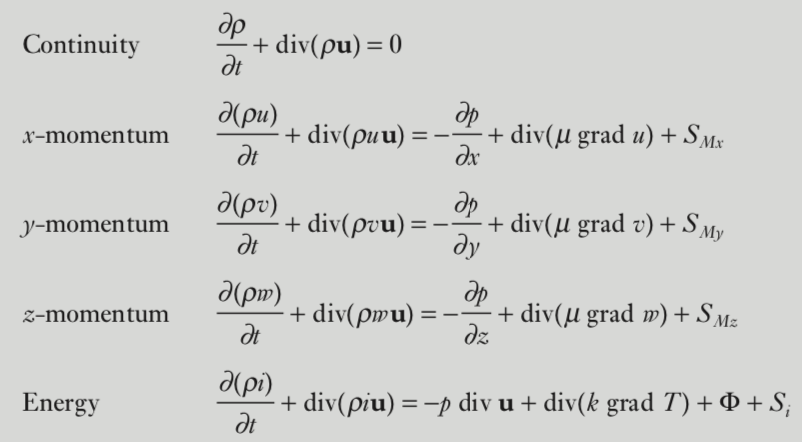
\includegraphics[scale=0.8]{5eq}
\end{figure}

$\rho = density$ \\
$t = time$ \\
$\mathbf{u} = flow vector$\\
$u = flow component in x-direction$ \\
$p = pressure$ \\
$\mu = dynamic viscosity$\\
$S_{Mx} = x-momentum source$ \\
$v = flow component in y-direction$ \\
$S_My = y-momentum source$ \\
$w = flow component in z-direction$ \\
$S_mz = z-momentum source$ \\
$i = internal energy$ \\
$k = thermal conductivity$ \\
$\Phi = dissipation function$ \\
$S_i = internal energy source$

(I don't know yet how to get space characters in functions)

Altogether we have 7 equations and 7 unknowns, giving us a closed system which can then be solved, initial and boundary conditions.

\subsection{Dissipation equation}

\begin{figure}[h]
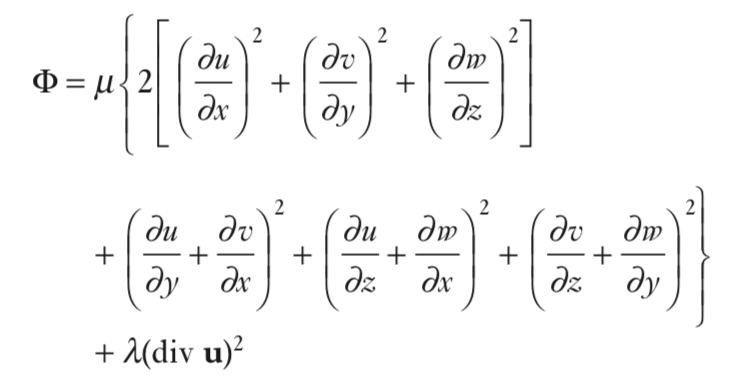
\includegraphics[scale=0.8]{dissipation}
\end{figure}
$\lambda = 2/3\mu$\\

\subsection{Equations of state}

The variables p and i  can be expressed as functions of density $\rho$ and temperature T. These functions are called the equations of state. In this project we will use an approximation where we use the ideal gas law as our equations of state:

$p = \rho RT$  and $i = C_{vT}$

$R = ideal gas constant$
$C_v = heat capacity$

Equation states assume thermodynamic equilibrium, i.e. that changes in temperature are slow enough that no significant temperature gradients appear throughout the model space.

Since we are dealing with air at low velocities, we will also assume incompressibility for our fluid. This allows us to decouple pressure (p) and density ($\rho$) so that density varies only due to temperature. 

\subsection{Continuity equation}

The continuity equation, also called the mass balance equation, is based off of conservation of mass (density in this case, since we're dealing with fixed volumes). It states that the change of mass in a volume is equal to the mass entering/leaving it via the flow.

\subsection{Momentum equations}

The three momentum equations in the x, y and z direction tell us that the rate of change in momentum in a certain direction in a volume is given by the momentum in that direction from fluid flowing into/out of the volume + the momentum in that direction given by pressure (the minus sign comes from pressure pushing in the opposite direction of its gradient) + the momentum in that direction applied by shear stresses + momentum in that direction applied by sources.

\subsection{Energy equation}

The energy equation tells us that the change rate of internal energy in a volume is equal to the internal energy from fluid flowing into/out of the volume + the potential energy from pressure it recieves/loses due to flow + the energy it recieves/loses due to thermal conductivity + the energy gained from deformation of the fluid converted into internal energy + energy from sources.

Gravity will be incorporated as an internal energy-source.

If the fluid is incompressible, $\rho$ and $i$ are uniform in space and div($\mathbf{u}$) = 0. This, together with the ideal gas law, allows us to simplify the energy equation into:

\begin{figure}[h]
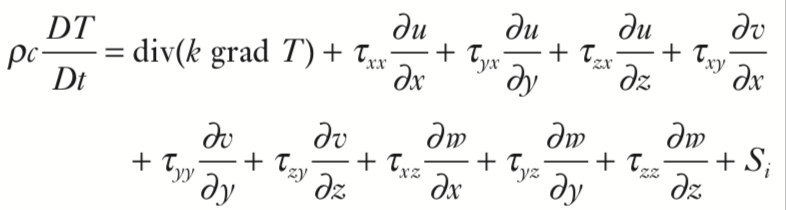
\includegraphics[scale=0.8]{newenergy}
\end{figure}

(the $\rho$ should be within the derivative since it in our case is time dependent. This allows use to convert $\rho T$ into p/R. Since we assume p is constant, its derivative over time will be 0 which means we get a left side that's 0)

\section{Transport equation}

Since we already have enough information to solve the flow of our model, we can now calculate the rate of change for specific attributes $\phi$ in the flow, through so-called transport equations.

\begin{figure}[h]
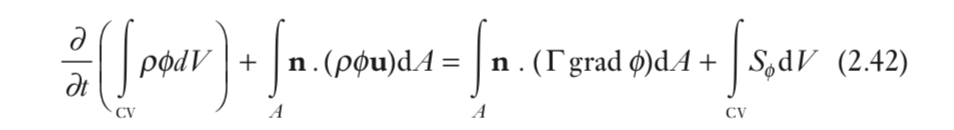
\includegraphics[scale=0.8]{navier}
\end{figure}

This equation says is that the $\phi$ gained in a unit volume $\phi$ leaving the unit volume through advection equals the $\phi$ entering the unit volume through diffusion plus the $\phi$ generated within the volume.

The same equation but time-dependent:
\\
\begin{figure}[h]
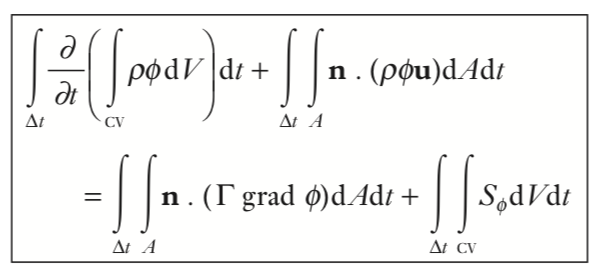
\includegraphics[scale=0.8]{naviertime}
\end{figure}
\\

Phi in our cases will be the species concentration of different chemical compounds found in an urban street environment.

\section{Turbulence}

\section{Radiation}

Radiation is the transmission of energy between bodies through space in the form of electromagnetic waves. No medium is required for this, which is why the radiative rays from the sun are able to reach the earth, despite there being no medium inbetween.

For a given body, incident radiative energy is either absorbed, reflected or transmitted, according to its \textbf{absorptivity} (a), \textbf{reflexivity} (r) and \textbf{transmissivity} ($\tau$) coefficients. These range from 0 to 1, and and have a sum equal to 1 due to the law of conservation of energy.

In most CFD cases, including this one, all boundary surfaces are opaque, meaning $\tau = 0$.

The equation for how much energy a radiative body emits is given by the Stefan-Boltzmann law:
\\
$j_r = A\epsilon \sigma_{SB}T^4$

A is the area of the body.

$\epsilon$ is the \textbf{emissivity} of the body. It is defined as the fraction of energy radiated from the body compared to the amount of energy that would be radiated by an ideal blackbody of equal surface area.

$\sigma$ is \textbf{Stefan-Boltzmann's constant}, defined as approximately $5.67*10^{-8}Wm^{-2}K^{-4}$.

T is the temperature of the body.

We can now set up an equation for the radiative energy contribution in a system:

$Sh()=aG-(\epsilon \sigma_{SB}T^4)$

Where G is equal to the incident radiative energy.

In other words, the radiatiative energy contribution to the energy equation is equal to the absorbed radiative energy (aG) minus the emitted radiative energy $(\epsilon \sigma_{SB}T^4)$. Looking at the energy equation function, this contribution can be found in the radiation->Sh(thermo) term.

\begin{verbatim}
     fvScalarMatrix hEqn(    
     fvm::div(phi, h)       
     - fvm::Sp(fvc::div(phi), h)
     - fvm::laplacian(turbulence->alphaEff(), h)      
     == fvc::div(phi/fvc::interpolate(rho)*fvc::interpolate(p))
     - p*fvc::div(phi/fvc::interpolate(rho))
     + radiation->Sh(thermo));
\end{verbatim}

To be able to solve the radiation contribution equation, the absorbptivity, emissivity and incident radiation G need to be modelled.

Absorbptivity and emissivity for a surface depend on wavelength, temperature and material. OpenFOAM has multiple functions to choose from, but for most intents and purposes a constant absoptivity/emissivity model suffices. The model can be set using the absorptionEmissionModel parameter in the \textbf{constant/radiationProperties} file.

G is trickier to model. The most widely used models are \textbf{S2S}, \textbf{FvDOM} and \textbf{P1}. They each implement the \textbf{Ru()} and \textbf{Rp()} functions, which are the constant and temperature-varying contributions to \textbf{Sh()}, respectively. We can see their use the in the \textbf{radiationModel::Sh()} function:

\begin{verbatim}
Foam::tmp<Foam::fvScalarMatrix> Foam::radiation::radiationModel::Sh
 (
     const basicThermo& thermo,
     const volScalarField& he
 ) const
 {
     const volScalarField Cpv(thermo.Cpv());
     const volScalarField T3(pow3(T_));
  
     return
     (
         Ru()
       - fvm::Sp(4.0*Rp()*T3/Cpv, he)
       - Rp()*T3*(T_ - 4.0*he/Cpv)
     );
 }
\end{verbatim}

The equation looks complicated at first glance, but the fvm::Sp() row and parts of the third row are simply an addition and subtraction of the same term in order to increase diagonal dominance. It's made more clear with the shifting of some terms:

$Sh() = Ru() - (4Rp*\frac{T^3h}{C_p}) - Rp()T^4 + (4Rp*\frac{T^3h}{C_p}) = Ru() - Rp()T^4$

The radiation models will in different ways calculate Ru() and Rp() in a way that makes Sh() represent our analytically derived $aG-(\epsilon \sigma_{SB}T^4)$ equation.

\subsection{viewFactor}

The viewFactor model calculates, for each boundary face of the mesh, a view factor coefficient for each other face in the mesh, determined by how "visible" the faces are to each other. The incident radiation for a face is then calculated by adding together the emitted radiative energy of all faces visible to that face, weighted by their view factor.

It assumes full transparency for the fluid and therefore gives no actual direct contribution to the radiation term of the energy equation. Instead it calculates qr, the boundary heat flux of the boundary patches, to be used in boundary condition equations of the mesh. In this way radiative energy is added to a cell through the $\nabla (\Gamma \nabla T)$ term rather than the radiationModel.Sh(thermo) term. The wall is only evaluated at the faces of the mesh. The model requires a lot of memory space to store the view factors, especially for finer meshes.

\subsection{FvDOM}

The FvDOM (Finite volume Discrete Ordinates Model) model divides emitted rays into a discrete number of solid angles, and solves them through ray-tracing. It is a computationally expensive but accurate radiation model.

\subsection{P1}

The P1 model simply assumes directional equilibrium between rays, and solves for the incident radiation as if it were a diffusive attribute. It works best for cases where the optical thickness (a * L) is high, i.e. where a substantial fraction of a beam's energy gets absorbed by the fluid before reaching a boundary.

It uses the following transport equation for G:

$\nabla * (\Gamma \nabla G) - aG + 4\epsilon \sigma T^4$

Which can found in the P1.C file as:

\begin{verbatim}
// Solve G transport equation
solve
(
    fvm::laplacian(gamma, G_)
    - fvm::Sp(a_, G_)
    ==
    - 4.0*(e_*physicoChemical::sigma*pow4(T_) ) - E_
);
\end{verbatim}

Here, \textbf{e\_} is the emmissivity, \textbf{sigma} is the Stefan-Boltzmann constant and \textbf{E\_} is the emission contribution.

Gamma is the "diffusive" coefficient for the P1 radiation, and is calculated in the following function:

\begin{verbatim}
// Construct diffusion
const volScalarField gamma
(
    IOobject
    (
        "gammaRad",
        G_.mesh().time().timeName(),
        G_.mesh(),
        IOobject::NO_READ,
        IOobject::NO_WRITE
    ),
    1.0/(3.0*a_ + sigmaEff + a0)
);
\end{verbatim}

here sigmaeff represents the scattering coefficient, which tells us how much ray intensity fades for each unit length travelled through the fluid.

\section{Solar load}

The solarLoad library, implemented for OpenFOAM+, is used to calculate the solar load on a CFD mesh. The direction of the sunbeams is set either to a constant direction or calculated with the included solarCalculator class. It also accounts for shading and reflexivity.

It can either act as a standalone radiation model or be added onto the viewFactor and FvDOM radiation models by setting \textbf{useSolarLoad} to \textbf{true} in \textbf{constant/radiationProperties}. The parameters for your solar model are then set in the \textbf{solarLoadCoeffs} dictionary in the same file. If combining solarLoad with FvDOM, you can only use one frequency band in the domain. When using the solarLoad model in conjunction with another model, it is only evaluated at boundary faces, not the internal field (similar to viewFactor).

\subsection{solarLoad.C}

Looking at solarLoad.C's Rp() function:

\begin{verbatim}
Foam::tmp<Foam::volScalarField> Foam::radiation::solarLoad::Rp() const
{
    return tmp<volScalarField>::New
    (
        IOobject
        (
            "Rp",
            mesh_.time().timeName(),
            mesh_,
            IOobject::NO_READ,
            IOobject::NO_WRITE,
            false
        ),
        mesh_,
        dimensionedScalar
        (
            dimMass/pow3(dimTime)/dimLength/pow4(dimTemperature),
            Zero
        )
    );
}
\end{verbatim}
We can see that its Rp() function returns zero. This is because the Rp() coefficient represents the part of the radiation contribution that scales with $T^4$. Since the sun's intensity depends on the sun and not on the temperatures within the mesh, the solarLoad model only contributes to the Ru() part of Sh().

The Ru value is calculated with the calculate() function:
\begin{verbatim}
void Foam::faceShading::calculate()
{

...

bool facesChanged = updateHitFaces();

...

updateDirectHitRadiation(hitFacesId, includeMappedPatchBasePatches);

...

updateSkyDiffusiveRadiation
        (
            includePatches,
            includeMappedPatchBasePatches
        );

...

if (useReflectedRays_)
        {
            updateReflectedRays(includeMappedPatchBasePatches);
        }
        
...

}
\end{verbatim}

It calls on 4 sub-functions, described below.

\subsubsection{updateHitFaces()}

This sub-function recalculates the sun's position and subsequently determines the boundary faces that are directly hit by sunlight based on the new position by calling hitFaces\_->correct(). The hit faces are stored in the hitFaces\_ object, which is an instance of the class faceShading, defined in faceShading.C.

\begin{verbatim}
bool Foam::radiation::solarLoad::updateHitFaces()
{

    ...
    
        if (updateIndex > updateTimeIndex_)
        {
            Info << "Updating Sun position..." << endl;
            updateTimeIndex_ = updateIndex;
            solarCalc_.correctSunDirection();
            hitFaces_->direction() = solarCalc_.direction();
            hitFaces_->correct();
            return true;
        }
        
    ...    
        
}
\end{verbatim}
\begin{verbatim}
void Foam::faceShading::correct()
{
    calculate();
}
\end{verbatim}
\begin{verbatim}
void Foam::faceShading::calculate()
{

    ...

        if (((direction_ & nf) > 0) && (t[faceI] == 0.0))
        {
            dynFacesI.append(faceI + pp.start());
            dynCf.append(cf[faceI]);
            nFaces++;
        }

    ...
    
\end{verbatim}

First all the faces whose normal vectors have a component facing the sun, determined by (direction\_ \& nf > 0) (\& is a dot product operator in OpenFOAM), and whose transparency equal 0, are collected.

\begin{verbatim}
    
    ...
    
    scalar maxBounding = 5.0*mag(mesh_.bounds().max() - mesh_.bounds().min());
    
    ...
    
    do
        {
            for (; i < Cfs.size(); i++)
            {
                const point& fc = Cfs[i];
    
                const label myFaceId = hitFacesIds[i];
    
                const vector d(direction_*maxBounding);
    
                start.append(fc - 0.001*d);
    
                startIndex.append(myFaceId);
    
                end.append(fc - d);
    
            }
    
        }while (returnReduce(i < Cfs.size(), orOp<bool>()));
        
    ...
\end{verbatim}

Here we, for each face that was stored earlier, store its center as a start point (or rather, the point just before the sun hits the center). Then we project a vector from that point towards the sun with a magnitude of approximately 5 times the diagonal of the mesh (direction\_*maxBounding), and store the point at the other end of that vector as the corresponding end point. startIndex helps the program remember which face the points correspond to.

\begin{verbatim}

    ...
    
        List<pointIndexHit> hitInfo(startIndex.size());
            surfacesMesh.findLine(start, end, hitInfo);
    
            // Collect the rays which has 'only one not wall' obstacle between
            // start and end.
            // If the ray hit itself get stored in dRayIs
            forAll(hitInfo, rayI)
            {
                if (!hitInfo[rayI].hit())
                {
                    rayStartFace.append(startIndex[rayI]);
                }
            }
            
    ...

}
\end{verbatim}

The surfacesMesh.findLine(start, end, hitInfo) function calculates, for every start and end point pair, if the line going from the start point to the end point ever intersects the mesh, and stores that information in hitInfo. In the forAll loop that follows, every face that has an unblocked path towards the sun is stored in rayStartFace. These faces get transferred to the public list rayStartFaces\_, which can be accessed by solarLoad.C.

\subsubsection{updateDirectHitRadiation()}

This sub-function calculates the heat flux contribution from direct solar exposure.

\begin{verbatim}
bool Foam::radiation::solarLoad::updateDirectHitRadiation()
{
    
    ...

        const vector qPrim =
            solarCalc_.directSolarRad()*solarCalc_.direction();

        const vectorField& n = pp.faceNormals();

        {
            qprimaryBf[patchID][localFaceI] +=
                (qPrim & n[localFaceI])
                * spectralDistribution_[bandI]
                * absorptivity_[patchID][bandI]()[localFaceI];
        }

        if (includeMappedPatchBasePatches[patchID])
        {
            qrBf[patchID][localFaceI] += qprimaryBf[patchID][localFaceI];
        }
        else
        {
            const vectorField& sf = mesh_.Sf().boundaryField()[patchID];
            const label cellI = pp.faceCells()[localFaceI];

            Ru_[cellI] +=
                (qPrim & sf[localFaceI])
              * spectralDistribution_[bandI]
              * absorptivity_[patchID][bandI]()[localFaceI]
              / V[cellI];
        }
\end{verbatim}

We will later find out how the solar calculator works. In the above code we can see that a vector representing sunlight, qPrim, is defined. It has the same direction as the sun, and the same magnitude as the solar intensity (directSolarRad()). Then, for each frequency band, each face of each patch gets added to it a heat flux value (qprimaryBf), equal to the dot product between the sun and the face normal, times the normalized spectral distribution of that band, times the absorptivity of that face for that band. The reason why a dot product with the face normal is used as a factor is to account for the angular visibility of the face.

The calculated flux then gets added either to the qr\_ variable (which qrBf references) or to the energy equation of the cells next to the walls, depending on settings set in the case files.

\subsubsection{updateSkyDiffusiveRadiation()}

This sub-function calculates the sky diffusive radiation contribution, which represents the radiation absorbed by the atmosphere and ground and then re-emitted in a diffuse manner throughout the mesh.

It is calculated differently depending on the solar model used. 

\begin{verbatim}
void Foam::radiation::solarLoad::updateSkyDiffusiveRadiation
(
    const labelHashSet& includePatches,
    const labelHashSet& includeMappedPatchBasePatches
)
{
    const polyBoundaryMesh& patches = mesh_.boundaryMesh();
    const scalarField& V = mesh_.V();
    volScalarField::Boundary& qrBf = qr_.boundaryFieldRef();

    switch(solarCalc_.sunLoadModel())
    {
        case solarCalculator::mSunLoadFairWeatherConditions:
        case solarCalculator::mSunLoadTheoreticalMaximum:
        {
            for (const label patchID : includePatches)
            {
                const polyPatch& pp = patches[patchID];
                const scalarField& sf = mesh_.magSf().boundaryField()[patchID];

                const vectorField n = pp.faceNormals();
                const labelList& cellIds = pp.faceCells();

                forAll(n, faceI)
                {
                    const scalar cosEpsilon(verticalDir_ & -n[faceI]);

                    scalar Ed(0.0);
                    scalar Er(0.0);
                    const scalar cosTheta(solarCalc_.direction() & -n[faceI]);

                    {
                        // Above the horizon
                        if (cosEpsilon == 0.0)
                        {
                            // Vertical walls
                            scalar Y(0);

                            if (cosTheta > -0.2)
                            {
                                Y = 0.55+0.437*cosTheta + 0.313*sqr(cosTheta);
                            }
                            else
                            {
                                Y = 0.45;
                            }
                            Ed = solarCalc_.C()*Y*solarCalc_.directSolarRad();
                        }
                        else
                        {
                            //Other than vertical walls
                            Ed =
                                solarCalc_.C()
                              * solarCalc_.directSolarRad()
                              * (1.0 + cosEpsilon)/2.0;
                        }

                        // Ground reflected
                        Er =
                            solarCalc_.directSolarRad()
                          * (solarCalc_.C() + Foam::sin(solarCalc_.beta()))
                          * solarCalc_.groundReflectivity()
                          * (1.0 - cosEpsilon)/2.0;
                    }

                    const label cellI = cellIds[faceI];
                    if (includeMappedPatchBasePatches[patchID])
                    {
                        for (label bandI = 0; bandI < nBands_; bandI++)
                        {
                            qrBf[patchID][faceI] +=
                                (Ed + Er)
                              * spectralDistribution_[bandI]
                              * absorptivity_[patchID][bandI]()[faceI];
                        }
                    }
                    else
                    {
                        for (label bandI = 0; bandI < nBands_; bandI++)
                        {
                            Ru_[cellI] +=
                                (Ed + Er)
                              * spectralDistribution_[bandI]
                              * absorptivity_[patchID][bandI]()[faceI]
                              * sf[faceI]/V[cellI];
                        }
                    }
                }
            }
        }
        break;
    }
\end{verbatim}

For the mSunLoadFairWeatherConditions and mSunLoadTheoreticalMaximum models, the model creates a cosEpsilon value for each face, being the dot product between the reversed face normal and the vector pointing towards the earth's core (in almost every case, the normalized g vector). Since both the reversed normal vector and the downwards pointing vector are normalized, the dot product will be equal to the cosine of the angle between them. This means that a face on the floor, whose reversed normal vector points downwards, will get the cosEpsilon value of cos(0) = 1. A vertical wall face, whose normal (and reverse normal) will always be at a 90 degree angle from the g vector, giving the face a cosEpsilon value of cos(90) = 0. Non-orthogonal faces will have a value inbetween 0 and 1. An exception to this are faces with a normal vector with a downwards facing component, which have a cosEpsilon value of [-1, 0).

Each face then gets assigned an Ed and an Er value, which each represent the diffusive radiance contribution from the sky and ground respectively. Their equations each feature a view factor. For sky diffusivity it equals (1.0 - cosEpsilon)/2.0 and ground for ground diffusivity it equals (1.0 - cosEpsilon)/2.0. They both range from 0 to 1, and add up to 1 for any one face. They can be seen as angle-dependent weights for a face. A face on the floor will have a ground diffusivity wieght of 0 and a sky diffusivity of 1, since it can only see the sky and not the ground.

Vertical faces get special treatment. Faces where cosTheta > -0.2, i.e. where the normal vector points somewhat away from the sun, i.e. significantly shaded faces, get a sky diffusive weight of 0.55+0.437*cosTheta + 0.313*sqr(cosTheta). Vertical faces somewhat pointing towards the sun are assigned a sky diffusive wieght of 0.45, slightly lower than the 0.5 they would have been assigned by the (1.0 + cosEpsilon)/2.0 function.

The diffusive radiation intensities for sky and ground diffusion are determined by the diffusive constant C, the solar intensity directSolarRad and the groundReflectivity, all defined at run-time in the solarLoadCoeffs dictionary.

The mSunLoadConstant model has a much simpler calculation:

\begin{verbatim}
        case solarCalculator::mSunLoadConstant:
        {
        
            ...
            
                {
                    for (label bandI = 0; bandI < nBands_; bandI++)
                    {
                        qrBf[patchID][faceI] +=
                            solarCalc_.diffuseSolarRad()
                          * spectralDistribution_[bandI]
                          * absorptivity_[patchID][bandI]()[faceI];
                    }
                }
                else
                {
                    for (label bandI = 0; bandI < nBands_; bandI++)
                    {
                        Ru_[cellI] +=
                            (
                                spectralDistribution_[bandI]
                              * absorptivity_[patchID][bandI]()[faceI]
                              * solarCalc_.diffuseSolarRad()
                            )*sf[faceI]/V[cellI];
                    }
                }
                
            ...   
                    
        }
    }
}
\end{verbatim}

Here, the user-defined diffusive solar irradiation intensity (diffuseSolarRad) is simply added on to walls directly in a uniform matter. The calculation is the same as in the updateDirectHitRadiation function, except there's no reduction of absorption based on the angle of exposure.

\subsubsection{updateReflectedRays()}

This sub-function calculates specular reflection with a depth of 1 bounce. It does so in a similar way to FvDOM, where only a discrete number of angles are available. Each time a bounce direction is calculated it selects the discrete angle that's as close to it as possible, and that becomes its actual direction.

\begin{verbatim}
void Foam::radiation::solarLoad::updateReflectedRays
(
    const labelHashSet& includePatches
)
{

    ...

        reflectedFaces_->correct();
        
    ...
\end{verbatim}

reflectedFaces is an instance of the faceReflecting class, defined in faceReflecting.C.

\begin{verbatim}
void Foam::faceShading::correct()
{
    calculate();
}
\end{verbatim}

\begin{verbatim}
void Foam::faceReflecting::correct()
{
    calculate();
}
\end{verbatim}

\begin{verbatim}
void Foam::faceReflecting::calculate()
{

    ...

        vector refDir =
            sunDir + 2.0*(-sunDir & n[faceI]) * n[faceI];

          // Look for the discrete direction
                    scalar dev(-GREAT);
                    label rayIndex = -1;
                    forAll(refDiscAngles_, iDisc)
    
            forAll(refDiscAngles_, iDisc)
                {
                    scalar dotProd = refDir & refDiscAngles_[iDisc];
                    if (dev < dotProd)
                    {
                        dev = dotProd;
                        rayIndex = iDisc;
                    }
                }
    
                if (rayIndex >= 0)
                {
                    if (refDisDirsIndex[rayIndex] == -1)
                    {
                        refDisDirsIndex[rayIndex] = 1;
                    }
                }
    
                refFacesDirIndex.insert
                (
                    globalNumbering.toGlobal(globalID),
                    rayIndex
                );
                        
    ...
    
\end{verbatim}

Here refDir is calculated as the exact reflection angle off the face. In the following forAll loop, each available discrete angle is gone through and compared to refDir. The angle whose dot product with refDir is the largest is stored as rayIndex. Since cos gets larger as it approaches 0, the discrete angle with the largest dot product will also have the smallest angle in reference to refDir. rayIndex then gets stored in refFacesDirIndex for later use.

\begin{verbatim}

    ...

    scalar maxBounding = 5.0*mag(mesh_.bounds().max() - mesh_.bounds().min());

    ...

        forAll(refDisDirsIndex, dirIndex)
                    {
                        if (refDisDirsIndex[dirIndex] > -1)
                        {
                            if ((nf & refDiscAngles_[dirIndex]) > 0)
                            {
                                const vector direction = -refDiscAngles_[dirIndex];
        
                                start.append(fc + 0.001*direction);
        
                                startIndex.append(myFaceId);
                                dirStartIndex.append(dirIndex);
        
                                end.append(fc + maxBounding*direction);
                            }
                        }
                    }
                }
        
            }while (returnReduce(i < Cfs_->size(), orOp<bool>()));
        
            List<pointIndexHit> hitInfo(startIndex.size());
        
            surfacesMesh_->findLine(start, end, hitInfo);
                        
    ...
    
\end{verbatim}

Here the faces hit by the reflected rays are determined in a similar way they were in updateDirectHits(), except here hitInfo isn't used to find the lines without intersections, but is instead used to find the faces it intersects with.


\subsection{solarCalculator}

The solarCalculator class keeps track of the sun direction and solar intensity. There are 2 models for direction and 3 for intensity. Direction is calculated in the calculateSundirection function, which uses the beta and theta angle variables, which are the sun angle above the horizon and the sun's cardinal angle in relation to the southern direction, respectively. These are calculated in the calculateBetaTheta function. The models for sun direction are:

\subsubsection{sunDirConstant}

Sun direction is set in the dictionary with the sunDirection entry.

\subsubsection{sunDirTracking}

Beta and theta are calculated from the following parameters:
\begin{itemize}
    \item localStandardMeridian : GMT (Local Zone Meridian) in hours
    \item startDay :  day from 1 to 365)
    \item startTime:  in hours
    \item longitude:  in degrees
    \item latitude:   in degrees
    \item gridUp:     grid orientation upwards
    \item gridEast    grid orientation eastwards
\end{itemize}
            
The parameters are specified in the solarLoadCoeffs dictionary.


As for intensity, the available models are:

\subsubsection{sunLoadConstant}

Solar intensity is set in the dictionary entries directSolarRad and diffuseSolarRad

\subsubsection{sunLoadFairWeatherConditions}

The solar intensity follows the Fair Weather Conditions Method from the ASHRAE Handbook. The entries are (taken from the comments of the source code):

\begin{itemize}
    \item skyCloudCoverFraction: Fraction of sky covered by clouds (0-1)
    \item A: Apparent solar irradiation at air mass m = 0
    \item B: Atmospheric extinction coefficient
    \item beta: Solar altitude (in degrees) above the horizontal plane. Is either entered or calculated
    \item groundReflectivity : Ground reflectivity
\end{itemize}

The direct solar flux is calculated as:

$directSolarRad = (1 - 0.75*skyCloudCoverFraction^3)*\frac{A}{exp(B/sin(beta)})$

\subsubsection{sunLoadTheoreticalMaximum}

The solar intensity is the same as for sunlight falling at a 0 degree angle with no cloud cover.

The entries are (taken from the source code comments):
\begin{itemize}
    \item Setrn
    \item SunPrime
    \item roundReflectivity
\end{itemize}
In this model the flux is calculated as: directSolarRad = Setrn*SunPrime

Sky diffusivity is calculated in the same way as in sunLoadFairWeatherConditions.

\section{Boundary conditions}

\subsection{Marshak Boundary Condition}

\subsection{externalWallHeatFluxTemperature}


% Chapter Template

\chapter{OpenFOAM} % Main chapter title

\label{openfoam} % Change X to a consecutive number; for referencing this chapter elsewhere, use \ref{ChapterX}


\section{UEqn}

.../reactingFoam/UEqn.H:

\begin{verbatim}
MRF.correctBoundaryVelocity(U);
 
 tmp<fvVectorMatrix> tUEqn
 (
     fvm::ddt(rho, U) + fvm::div(phi, U)
   + MRF.DDt(rho, U)
   + turbulence->divDevRhoReff(U)
  ==
     fvOptions(rho, U)
 );
 fvVectorMatrix& UEqn = tUEqn.ref();
 
 UEqn.relax();
 
 fvOptions.constrain(UEqn);
 
 if (pimple.momentumPredictor())
 {
     solve(UEqn == -fvc::grad(p));
 
     fvOptions.correct(U);
     K = 0.5*magSqr(U);
 }
\end{verbatim} 
\vspace{\baselineskip}
The tmp wrapper has to do with optimizing the code for decreasing peak memory usage. Normally when C++ returns an object, it copies the object, returns the copy and deletes the original. This means that for a brief moment you have 2 data objects at the same time, which for complex grids can take a lot of memory. By wrapping large data structures in a tmp<Type> wrapper with a reference to the data, one overwrites the constructor and destructor of the object so that when the object is returned, a copy of the reference is created instead of a copy of the object itself. After returning the reference, the original pointer is dereferenced.
\vspace{\baselineskip}
MRF stands for multiple reference field, and has to do with rotational phenomena like fans and golf balls. The terms involving MRF need not be applied for our purposes.
\vspace{\baselineskip}
Looking at the fvm::ddt(rho, U) term, fvm:: means that it expresses the sought after term $\frac{d \rho \textbf{u}}{dt}$ in an implicit way, returning a matrix of coefficients. This is unlike functions in the fvc$::$ namespace, which return sought after values explicitly (by evaluating source terms or predicted terms).
\vspace{\baselineskip}
First we take a look at the turbulence->divDevRhoReff function. It returns the density times the effective viscous stress contribution to the momentum equation. Its implementation depends on the turbulence model chosen. To keep things simple I will look at the version implemented in linearViscousStress.C:
\vspace{\baselineskip}
\begin{verbatim}
 Foam::linearViscousStress<BasicTurbulenceModel>::divDevRhoReff
 (
     volVectorField& U
 ) const
 {
     return
     (
       - fvc::div((this->alpha_*this->rho_*this->nuEff())*dev2(T(fvc::grad(U))))
       - fvm::laplacian(this->alpha_*this->rho_*this->nuEff(), U)
     );
 }
\end{verbatim}
Alpha\_ is phase fraction, which for single phase solvers like reactionFoam is equal to 1.
\vspace{\baselineskip}
For the viscosity, $\mu_{eff} = \mu_t + \mu$. $\mu_t$ is calculated based on the turbulence model, and $\mu$ is typically read from the input file.
\vspace{\baselineskip}
dev stands for \textbf{deviatory}, and is defined by $dev(A) = A - \frac{1}{3}*tr(A)I$. dev2 is a slight modification, where $dev2(A) = A - \frac{2}{3}*tr(A)I$.
\vspace{\baselineskip}
From this, divDevRhoEff translates into:

\begin{figure}[H]
\centering
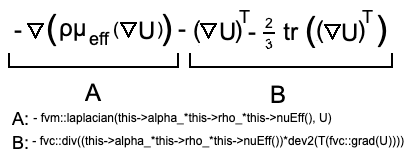
\includegraphics[scale=0.8]{divdevrhoreff}
\end{figure}

In the book (page 23), one equation for the viscous stress in the x-direction is:

\begin{figure}[H]
\centering
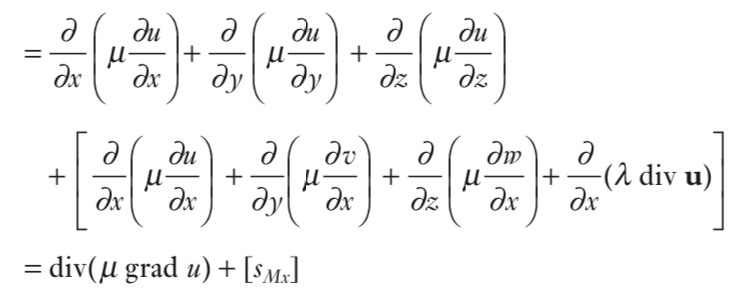
\includegraphics[scale=0.8]{viscous}
\end{figure}

Where $\lambda = -\frac{2}{3}\mu$ (an approximation commonly used for gaseous liquids). Similar equations can be derived for the y- and z-directions.
\vspace{\baselineskip}
For our momentum gradient matrix we have:
\begin{figure}[H]
\centering
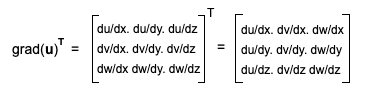
\includegraphics[scale=0.8]{gradUT}
\end{figure}

We can see that the first row of $grad(U)^T$ (corresponding to the shear stress in the x-direction) matches the gradients in the $[S_{Mx}]$ part of the equation.
\vspace{\baselineskip}
The $\frac{d}{dx}$ operator (and corresponding operators for the other directions) in $\frac{d}{dx}(\lambda div(\textbf{u}))$ term makes it so that only the diagonal of $grad(\textbf{u})^T$ is subtracted from.
\vspace{\baselineskip}
Since $div(U)=\frac{du}{dx} + \frac{dv}{dy} + \frac{dw}{dz} tr(grad(U)^T)$ we can now express $[S_{M}]$ (for all three directions) as $div(\mu grad(U)^T - \frac{2}{3} tr( \mu div(U)) = \mu dev2( grad(U)^T)$. $\mu$ can be moved outside of the matrix due to dev being a linear operator.
\vspace{\baselineskip}
We can clearly see this being represented in code through the line
\begin{verbatim}
- fvc::div((this->alpha_*this->rho_*this->nuEff())*dev2(T(fvc::grad(U))))
\end{verbatim}
while the $div(\mu grad(\textbf{u})$ term in the viscous part of the momentum equation is represented by
\begin{verbatim}
- fvm::laplacian(this->alpha_*this->rho_*this->nuEff(), U)
\end{verbatim}
The minus signs come from them being moved from the RHS in the book to the LHS in the solver.
\vspace{\baselineskip}
The multiplication with $\rho$ is in order to convert from kinematic to dynamic viscosity.
\vspace{\baselineskip}
Lastly I'm not sure why the first term is calculated explicitly while the second term is calculated explicitly.
\vspace{\baselineskip}
-----------
\vspace{\baselineskip}
Going back to the momentum equation, if we include the pressure correction (\begin{verbatim}solve(UEqn == -fvc::grad(p)); \end{verbatim} we get the following equation:

\begin{figure}[H]
\centering
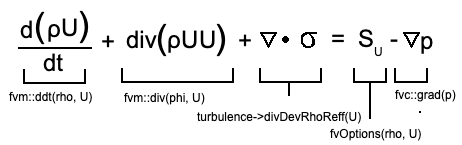
\includegraphics[scale=0.8]{momentumE}
\end{figure}

Where $\sigma$ is the newtonian stress tensor.
\vspace{\baselineskip}
After moving some terms to the RHS, it becomes almost exactly the momentum equation from the book.

\begin{figure}[H]
\centering
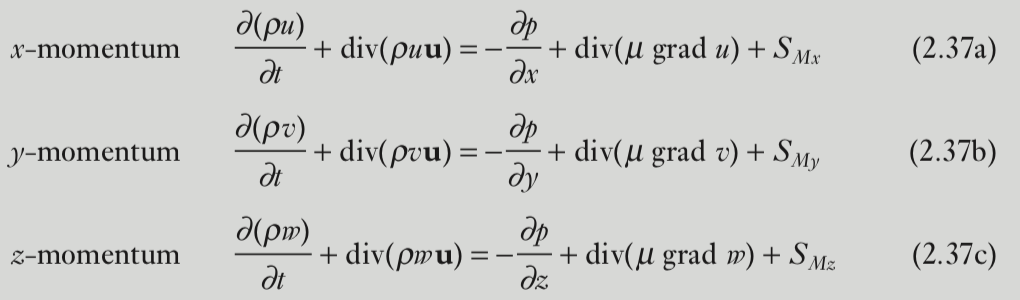
\includegraphics[scale=0.8]{momentumbook}
\end{figure}

UEqn.relax() constrains the magnitude of change in U compared to $U_0$ below a certain value, depending on the relaxation factors specified in fvSolutions.
\vspace{\baselineskip}
fvOptions.constrain(UEqn) adds user-specified boundary conditions (for example, the inlet patch must always have a flow of (3 0 0), or U cannot exceed 200 in magnitude), set in fvOptions.
\vspace{\baselineskip}
Since p was used explicitly in the equation it has not been updated since the last timestep, and does not satisfy the continuity equation with the new U matrix. fvOptions.correct(U) adjusts p with the new U so that the continuation equation is once again satisfied. 
\vspace{\baselineskip}
The line K = 0.5*magSqr(U) sets the kinematic velocity K to $0.5*U^2$.
\vspace{\baselineskip}
Since reactingFoam uses the pimple algorithm, U is not solved fully at every loop iteration, only when pimple.momentumPredictor() = true. For when the predictor is set to false, the velocity is only calculated in the PEqn.C file, at the line:
\vspace{\baselineskip}
U = HbyA - rAU*fvc::grad(p);

\section{pEqn}

.../reactingFoam/pEqn.H:
\begin{verbatim}
    rho = thermo.rho();
 
 volScalarField rAU(1.0/UEqn.A());
 surfaceScalarField rhorAUf("rhorAUf", fvc::interpolate(rho*rAU));
 volVectorField HbyA(constrainHbyA(rAU*UEqn.H(), U, p));
 
 if (pimple.nCorrPiso() <= 1)
 {
     tUEqn.clear();
 }
 
 ...
 
 {
     surfaceScalarField phiHbyA
     (
         "phiHbyA",
         (
             fvc::flux(rho*HbyA)
           + MRF.zeroFilter(rhorAUf*fvc::ddtCorr(rho, U, phi))
         )
     );
 
     MRF.makeRelative(fvc::interpolate(rho), phiHbyA);
 
     // Update the pressure BCs to ensure flux consistency
     constrainPressure(p, rho, U, phiHbyA, rhorAUf, MRF);
 
     while (pimple.correctNonOrthogonal())
     {
         fvScalarMatrix pEqn
         (
             fvm::ddt(psi, p)
           + fvc::div(phiHbyA)
           - fvm::laplacian(rhorAUf, p)
          ==
             fvOptions(psi, p, rho.name())
         );
 
         pEqn.solve();
 
         if (pimple.finalNonOrthogonalIter())
         {
             phi = phiHbyA + pEqn.flux();
         }
     }
 }
 
 #include "rhoEqn.H"
 #include "compressibleContinuityErrs.H"
 
 // Explicitly relax pressure for momentum corrector
 p.relax();
 
 U = HbyA - rAU*fvc::grad(p);
 U.correctBoundaryConditions();
 fvOptions.correct(U);
 K = 0.5*magSqr(U);
 
 if (pressureControl.limit(p))
 {
     p.correctBoundaryConditions();
     rho = thermo.rho();
 }
 
 if (thermo.dpdt())
 {
     dpdt = fvc::ddt(p);
 }
\end{verbatim}

(There is also a pcEqn.H, which will be excecuted if pimple is set to consistent. I will not go through it here.)
\vspace{\baselineskip}
The PEqn.H file first solves the pressure p iteratively and predicts the velocity U in accordance with the PISO loop. Through the momentum equation we can build the velocity coefficient matrix M, where \textbf{MU} = $-\nabla p$. From this the following matrices are defined:
\\\\
A = diag(M) \\
H = AU - MU \\
$rAU = A^{-1}$ \\
rhorAUf = $\rho A^{-1}$ (evaluated at the faces)
HbyA = $A^{-1}H$
phiHbyA = flux(rho*HbyA)
\vspace{\baselineskip}
A represents the pressure contribution from the velocity of a cell.
H represents the pressure contributions from the velocity neighboring cells.
\vspace{\baselineskip}
Let's take a look at the pressure correction loop:

\begin{verbatim}
    while (pimple.correctNonOrthogonal())
     {
         fvScalarMatrix pEqn
         (
             fvm::ddt(psi, p)
           + fvc::div(phiHbyA)
           - fvm::laplacian(rhorAUf, p)
          ==
             fvOptions(psi, p, rho.name())
         );
 
         pEqn.solve();
 
         if (pimple.finalNonOrthogonalIter())
         {
             phi = phiHbyA + pEqn.flux();
         }
     }
\end{verbatim}
The loop will iterate an amount of times based on how orthogonal the matrix is, in order to iteratively calculate the fluxes. For fully orthogonal matrices, it will only execute once. For each iteration, the term fvc::div(phiHbyA) will change, since it is calculated explicitly and depends on p.
\vspace{\baselineskip}
psi = $\psi = \frac{rho}{p}$, meaning the ddt term is basically just $\frac{d \rho}{dt}$
\vspace{\baselineskip}
Note that since we are solving for $\nabla p$, which depends on the flux on cell faces, we are first solving for cell faces rather than cell centers. Because of this, our terms are multiplied by $\rho$ to keep consistency with the continuity equation when calculating the divergence of phiHbyA.
\vspace{\baselineskip}
Solving for the Laplacian term we get:

\begin{figure}[H]
\centering
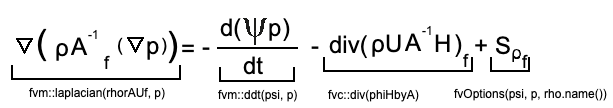
\includegraphics[scale=0.6]{pressurecode}
\end{figure}

This looks similar to the equation at the bottom of page 8 in the "A low-Mach number solver for variable density flows" paper:

\begin{figure}[H]
\centering
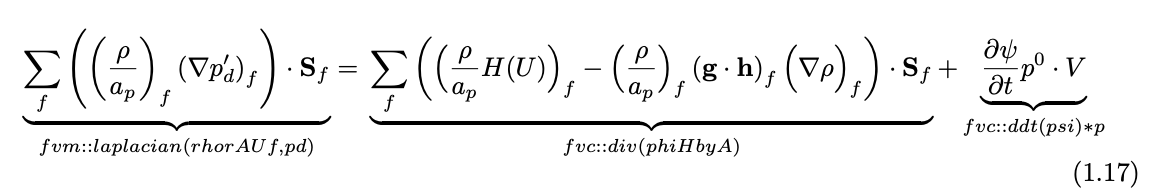
\includegraphics[scale=0.6]{pressuref}
\end{figure}

Since our equation came from the standard reactingFoam solver and not the buoyant one, and since the solver doesn't use a low-mach approximation, the gh term is missing and the pressure terms are slightly different.
\vspace{\baselineskip}
If you follow page 8 of that paper from bottom to top you will find how to derive this discretized version of the equation:

\begin{figure}[H]
\centering
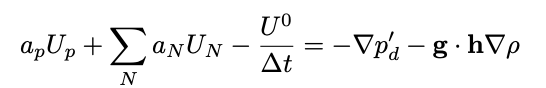
\includegraphics[scale=0.8]{disc}
\end{figure}

//(I will write my own derivation with my own pictures during the christmas break) \\
\vspace{\baselineskip}
Since $a_p U_p = AU$ and \[ \sum_{n=1} a_N U_N - \frac{U^0}{\delta t} = -H \], together with the fact that AU - H = MU, we get that MU = -$\nabla p$.
\vspace{\baselineskip}
After the pressure has been calculated, the density is calculated using the continuity equation. Then the new pressure is used to calculate a new U vector, by setting
\begin{verbatim}
    U = HbyA - RAU*fvc::grad(p);
\end{verbatim}
Constraints are enforced, the pressure is corrected and the kinetic energy K is adjusted. Next limits for pressure are checked, and lastly, unless dpdt is turned off (in the thermophysical properties file) the dpdt term is calculated.

\section{EEqn}

.../reactingFoam/EEqn.H:
\begin{verbatim}
    {
     volScalarField& he = thermo.he();
 
     fvScalarMatrix EEqn
     (
         fvm::ddt(rho, he) + mvConvection->fvmDiv(phi, he)
       + fvc::ddt(rho, K) + fvc::div(phi, K)
       + (
             he.name() == "e"
           ? fvc::div
             (
                 fvc::absolute(phi/fvc::interpolate(rho), U),
                 p,
                 "div(phiv,p)"
             )
           : -dpdt
         )
       - fvm::laplacian(turbulence->alphaEff(), he)
      ==
         reaction->Qdot()
       + fvOptions(rho, he)
     );
 
     EEqn.relax();
 
     fvOptions.constrain(EEqn);
 
     EEqn.solve();
 
     fvOptions.correct(he);
 
     thermo.correct();
 
     Info<< "min/max(T) = "
         << min(T).value() << ", " << max(T).value() << endl;
 }
\end{verbatim}

Assuming we are using the enthalpy energy equation, where he.name() == "h" and therefore the fifth term being equal to dpdt, we can set up the equation in the following way:

\begin{figure}[H]
\centering
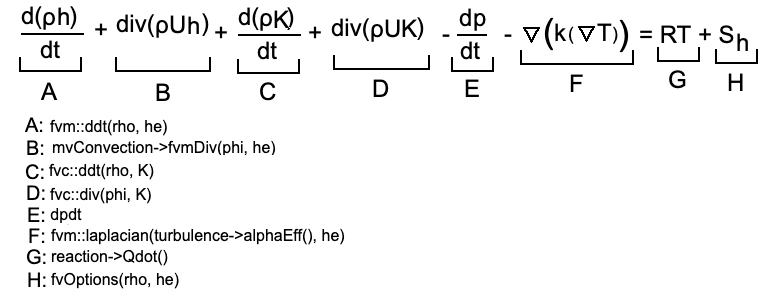
\includegraphics[scale=0.4]{energycode}
\end{figure}

Where RT is the temperature gained from chemical reactions.
Since $h_0 = h + K$ we have $\frac{d \rho h}{dt} + \frac{d \rho K}{dt} = \frac{d \rho h_0}{dt}$ and $div(h) + div(K) = div(h_0)$
\vspace{\baselineskip}
Moving the -dpdt term and the diffusive term to the RHS we get:

\begin{figure}[H]
\centering
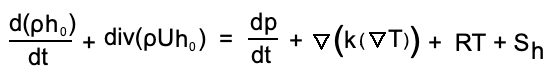
\includegraphics[scale=0.6]{energycode2}
\end{figure}

This is similar to the total enthalpy equation in the book:
\begin{figure}[H]
\centering
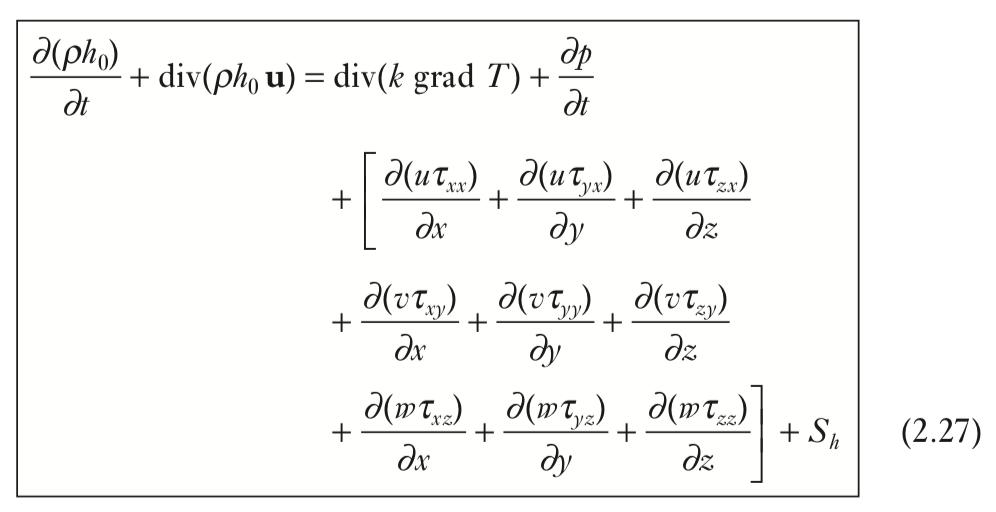
\includegraphics[scale=0.5]{enthalpytot}
\end{figure}
except that the dissipation term has been ignored and we have an extra reaction term RT.
\vspace{\baselineskip}
$\frac{dK}{dt}$ and div(K) are calculated explicitly since they only depend on the U matrix which is already solved in UEqn.H. The diffusive term depends on temperature which is solved alongside the enthalpy, and therefore needs to be solved implicitly.

\section{YEqn}

.../reactingFoam/YEqn.H:
\begin{verbatim}
 tmp<fv::convectionScheme<scalar>> mvConvection
 (
     fv::convectionScheme<scalar>::New
     (
         mesh,
         fields,
         phi,
         mesh.divScheme("div(phi,Yi_h)")
     )
 );
 
 {
     reaction->correct();
     volScalarField Yt(0.0*Y[0]);
 
     forAll(Y, i)
     {
         if (i != inertIndex && composition.active(i))
         {
             volScalarField& Yi = Y[i];
 
             fvScalarMatrix YiEqn
             (
                 fvm::ddt(rho, Yi)
               + mvConvection->fvmDiv(phi, Yi)
               - fvm::laplacian(turbulence->muEff(), Yi)
              ==
                 reaction->R(Yi)
               + fvOptions(rho, Yi)
             );
 
             YiEqn.relax();
 
             fvOptions.constrain(YiEqn);
 
             YiEqn.solve("Yi");
 
             fvOptions.correct(Yi);
 
             Yi.max(0.0);
             Yt += Yi;
         }
     }
 
     Y[inertIndex] = scalar(1) - Yt;
     Y[inertIndex].max(0.0);
 }
\end{verbatim}

inertIndex represents the index for inert mass, i.e. the fluid molecules that are not explicit components in any reaction, but might act as energy receptors for the reactions of other molecules. In this case, it will represent all molecules found in air except $OH, CH_4, O_2, O_3, NO and NO_2$.
\vspace{\baselineskip}
Yi represents the mass fraction of a certain species, that is $\frac{\rho_i}{\rho}$.
\vspace{\baselineskip}
Setting up the equation:

\begin{figure}[H]
\centering
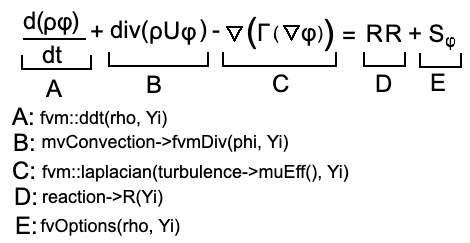
\includegraphics[scale=0.8]{transportcode}
\end{figure}

We can easily see how it resembles the scalar transport equation from the book:
\begin{figure}[H]
\centering
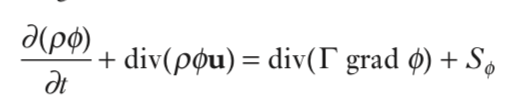
\includegraphics[scale=0.7]{transport}
\end{figure}
The only difference is the reaction->R(Yi) term, which represents the reaction source RR.


% Chapter Template

\chapter{Methodology} % Main chapter title

\label{methodology} % Change X to a consecutive number; for referencing this chapter elsewhere, use \ref{ChapterX}

%----------------------------------------------------------------------------------------
%	SECTION 1
%----------------------------------------------------------------------------------------
The open source program OpenFOAM will be used for the physical simulation of the street canyon. Existing modules for chemical reactions, solar irradiation, heat transfer and buoyancy exist in the OpenFOAM framework. A new solver will be created based on the rhoReactingBuoyantFoam solver, a standard solver in OpenFOAM, incorporating the externalSolarLoad library and chemical model supplied by the group from the Combustion Physics department. In order to properly program the solver and post process the data extensive knowledge of the mechanics of the program and utilized libraries must be attained.

After a base setup has been created in accordance with previous papers (in particular Zhang et al. (2019)\cite{zhang2019}), multiple configurations will be run in order to quantify the effects of certain parameters on the final $O_3$ and $NO_x$ concentrations. Radiation parameters and canyon width will be of special interest. As a post-processing tool ParaFOAM will be used.

\section{Implementation of Photolytic Solver}

Nunc posuere quam at lectus tristique eu ultrices augue venenatis. Vestibulum ante ipsum primis in faucibus orci luctus et ultrices posuere cubilia Curae; Aliquam erat volutpat. Vivamus sodales tortor eget quam adipiscing in vulputate ante ullamcorper. Sed eros ante, lacinia et sollicitudin et, aliquam sit amet augue. In hac habitasse platea dictumst.

%-----------------------------------
%	SUBSECTION 1
%-----------------------------------
\section{Simulation Setup}

Morbi rutrum odio eget arcu adipiscing sodales. Aenean et purus a est pulvinar pellentesque. Cras in elit neque, quis varius elit. Phasellus fringilla, nibh eu tempus venenatis, dolor elit posuere quam, quis adipiscing urna leo nec orci. Sed nec nulla auctor odio aliquet consequat. Ut nec nulla in ante ullamcorper aliquam at sed dolor. Phasellus fermentum magna in augue gravida cursus. Cras sed pretium lorem. Pellentesque eget ornare odio. Proin accumsan, massa viverra cursus pharetra, ipsum nisi lobortis velit, a malesuada dolor lorem eu neque.

%-----------------------------------
%	SUBSECTION 2
%-----------------------------------

\subsection{Mesh}


%----------------------------------------------------------------------------------------
%	SECTION 2
%----------------------------------------------------------------------------------------

\subsection{Turbulence Parameters}

Sed ullamcorper quam eu nisl interdum at interdum enim egestas. Aliquam placerat justo sed lectus lobortis ut porta nisl porttitor. Vestibulum mi dolor, lacinia molestie gravida at, tempus vitae ligula. Donec eget quam sapien, in viverra eros. Donec pellentesque justo a massa fringilla non vestibulum metus vestibulum. Vestibulum in orci quis felis tempor lacinia. Vivamus ornare ultrices facilisis. Ut hendrerit volutpat vulputate. Morbi condimentum venenatis augue, id porta ipsum vulputate in. Curabitur luctus tempus justo. Vestibulum risus lectus, adipiscing nec condimentum quis, condimentum nec nisl. Aliquam dictum sagittis velit sed iaculis. Morbi tristique augue sit amet nulla pulvinar id facilisis ligula mollis. Nam elit libero, tincidunt ut aliquam at, molestie in quam. Aenean rhoncus vehicula hendrerit.

\subsection{Radiation Parameters}

Sed ullamcorper quam eu nisl interdum at interdum enim egestas. Aliquam placerat justo sed lectus lobortis ut porta nisl porttitor. Vestibulum mi dolor, lacinia molestie gravida at, tempus vitae ligula. Donec eget quam sapien, in viverra eros. Donec pellentesque justo a massa fringilla non vestibulum metus vestibulum. Vestibulum in orci quis felis tempor lacinia. Vivamus ornare ultrices facilisis. Ut hendrerit volutpat vulputate. Morbi condimentum venenatis augue, id porta ipsum vulputate in. Curabitur luctus tempus justo. Vestibulum risus lectus, adipiscing nec condimentum quis, condimentum nec nisl. Aliquam dictum sagittis velit sed iaculis. Morbi tristique augue sit amet nulla pulvinar id facilisis ligula mollis. Nam elit libero, tincidunt ut aliquam at, molestie in quam. Aenean rhoncus vehicula hendrerit.

\subsection{Discretization schemes}

Sed ullamcorper quam eu nisl interdum at interdum enim egestas. Aliquam placerat justo sed lectus lobortis ut porta nisl porttitor. Vestibulum mi dolor, lacinia molestie gravida at, tempus vitae ligula. Donec eget quam sapien, in viverra eros. Donec pellentesque justo a massa fringilla non vestibulum metus vestibulum. Vestibulum in orci quis felis tempor lacinia. Vivamus ornare ultrices facilisis. Ut hendrerit volutpat vulputate. Morbi condimentum venenatis augue, id porta ipsum vulputate in. Curabitur luctus tempus justo. Vestibulum risus lectus, adipiscing nec condimentum quis, condimentum nec nisl. Aliquam dictum sagittis velit sed iaculis. Morbi tristique augue sit amet nulla pulvinar id facilisis ligula mollis. Nam elit libero, tincidunt ut aliquam at, molestie in quam. Aenean rhoncus vehicula hendrerit.

\subsection{Timestep}

Sed ullamcorper quam eu nisl interdum at interdum enim egestas. Aliquam placerat justo sed lectus lobortis ut porta nisl porttitor. Vestibulum mi dolor, lacinia molestie gravida at, tempus vitae ligula. Donec eget quam sapien, in viverra eros. Donec pellentesque justo a massa fringilla non vestibulum metus vestibulum. Vestibulum in orci quis felis tempor lacinia. Vivamus ornare ultrices facilisis. Ut hendrerit volutpat vulputate. Morbi condimentum venenatis augue, id porta ipsum vulputate in. Curabitur luctus tempus justo. Vestibulum risus lectus, adipiscing nec condimentum quis, condimentum nec nisl. Aliquam dictum sagittis velit sed iaculis. Morbi tristique augue sit amet nulla pulvinar id facilisis ligula mollis. Nam elit libero, tincidunt ut aliquam at, molestie in quam. Aenean rhoncus vehicula hendrerit.

\section{Resources}

Computers at the Department of Energy Sciences will be used in this case. For cases which require high computational power, resources provided by the Swedish National Infrastructure for Computing (SNIC) at PDC (Beskow) will be used. OpenFOAM and external libraries used are open source and freely available on the web. For the duration of the project an office desk and computer are supplied for the student at the K faculty building at LTH.
% Chapter Template

\chapter{Simulation} % Main chapter title

\label{simulation} % Change X to a consecutive number; for referencing this chapter elsewhere, use \ref{ChapterX}

%----------------------------------------------------------------------------------------
%	SECTION 1
%----------------------------------------------------------------------------------------

\section{Main Section 1}

Lorem ipsum dolor sit amet, consectetur adipiscing elit. Aliquam ultricies lacinia euismod. Nam tempus risus in dolor rhoncus in interdum enim tincidunt. Donec vel nunc neque. In condimentum ullamcorper quam non consequat. Fusce sagittis tempor feugiat. Fusce magna erat, molestie eu convallis ut, tempus sed arcu. Quisque molestie, ante a tincidunt ullamcorper, sapien enim dignissim lacus, in semper nibh erat lobortis purus. Integer dapibus ligula ac risus convallis pellentesque.

%-----------------------------------
%	SUBSECTION 1
%-----------------------------------
\subsection{Subsection 1}

Nunc posuere quam at lectus tristique eu ultrices augue venenatis. Vestibulum ante ipsum primis in faucibus orci luctus et ultrices posuere cubilia Curae; Aliquam erat volutpat. Vivamus sodales tortor eget quam adipiscing in vulputate ante ullamcorper. Sed eros ante, lacinia et sollicitudin et, aliquam sit amet augue. In hac habitasse platea dictumst.

%-----------------------------------
%	SUBSECTION 2
%-----------------------------------

\subsection{Subsection 2}
Morbi rutrum odio eget arcu adipiscing sodales. Aenean et purus a est pulvinar pellentesque. Cras in elit neque, quis varius elit. Phasellus fringilla, nibh eu tempus venenatis, dolor elit posuere quam, quis adipiscing urna leo nec orci. Sed nec nulla auctor odio aliquet consequat. Ut nec nulla in ante ullamcorper aliquam at sed dolor. Phasellus fermentum magna in augue gravida cursus. Cras sed pretium lorem. Pellentesque eget ornare odio. Proin accumsan, massa viverra cursus pharetra, ipsum nisi lobortis velit, a malesuada dolor lorem eu neque.

%----------------------------------------------------------------------------------------
%	SECTION 2
%----------------------------------------------------------------------------------------

\section{Main Section 2}

Sed ullamcorper quam eu nisl interdum at interdum enim egestas. Aliquam placerat justo sed lectus lobortis ut porta nisl porttitor. Vestibulum mi dolor, lacinia molestie gravida at, tempus vitae ligula. Donec eget quam sapien, in viverra eros. Donec pellentesque justo a massa fringilla non vestibulum metus vestibulum. Vestibulum in orci quis felis tempor lacinia. Vivamus ornare ultrices facilisis. Ut hendrerit volutpat vulputate. Morbi condimentum venenatis augue, id porta ipsum vulputate in. Curabitur luctus tempus justo. Vestibulum risus lectus, adipiscing nec condimentum quis, condimentum nec nisl. Aliquam dictum sagittis velit sed iaculis. Morbi tristique augue sit amet nulla pulvinar id facilisis ligula mollis. Nam elit libero, tincidunt ut aliquam at, molestie in quam. Aenean rhoncus vehicula hendrerit.
% Chapter Template

\chapter{Conclusion} % Main chapter title

\label{conclusion} % Change X to a consecutive number; for referencing this chapter elsewhere, use \ref{ChapterX}

%----------------------------------------------------------------------------------------
%	SECTION 1
%----------------------------------------------------------------------------------------

\section{Main Section 1}

Lorem ipsum dolor sit amet, consectetur adipiscing elit. Aliquam ultricies lacinia euismod. Nam tempus risus in dolor rhoncus in interdum enim tincidunt. Donec vel nunc neque. In condimentum ullamcorper quam non consequat. Fusce sagittis tempor feugiat. Fusce magna erat, molestie eu convallis ut, tempus sed arcu. Quisque molestie, ante a tincidunt ullamcorper, sapien enim dignissim lacus, in semper nibh erat lobortis purus. Integer dapibus ligula ac risus convallis pellentesque.

%-----------------------------------
%	SUBSECTION 1
%-----------------------------------
\subsection{Subsection 1}

Nunc posuere quam at lectus tristique eu ultrices augue venenatis. Vestibulum ante ipsum primis in faucibus orci luctus et ultrices posuere cubilia Curae; Aliquam erat volutpat. Vivamus sodales tortor eget quam adipiscing in vulputate ante ullamcorper. Sed eros ante, lacinia et sollicitudin et, aliquam sit amet augue. In hac habitasse platea dictumst.

%-----------------------------------
%	SUBSECTION 2
%-----------------------------------

\subsection{Subsection 2}
Morbi rutrum odio eget arcu adipiscing sodales. Aenean et purus a est pulvinar pellentesque. Cras in elit neque, quis varius elit. Phasellus fringilla, nibh eu tempus venenatis, dolor elit posuere quam, quis adipiscing urna leo nec orci. Sed nec nulla auctor odio aliquet consequat. Ut nec nulla in ante ullamcorper aliquam at sed dolor. Phasellus fermentum magna in augue gravida cursus. Cras sed pretium lorem. Pellentesque eget ornare odio. Proin accumsan, massa viverra cursus pharetra, ipsum nisi lobortis velit, a malesuada dolor lorem eu neque.

%----------------------------------------------------------------------------------------
%	SECTION 2
%----------------------------------------------------------------------------------------

\section{Main Section 2}

Sed ullamcorper quam eu nisl interdum at interdum enim egestas. Aliquam placerat justo sed lectus lobortis ut porta nisl porttitor. Vestibulum mi dolor, lacinia molestie gravida at, tempus vitae ligula. Donec eget quam sapien, in viverra eros. Donec pellentesque justo a massa fringilla non vestibulum metus vestibulum. Vestibulum in orci quis felis tempor lacinia. Vivamus ornare ultrices facilisis. Ut hendrerit volutpat vulputate. Morbi condimentum venenatis augue, id porta ipsum vulputate in. Curabitur luctus tempus justo. Vestibulum risus lectus, adipiscing nec condimentum quis, condimentum nec nisl. Aliquam dictum sagittis velit sed iaculis. Morbi tristique augue sit amet nulla pulvinar id facilisis ligula mollis. Nam elit libero, tincidunt ut aliquam at, molestie in quam. Aenean rhoncus vehicula hendrerit.

%----------------------------------------------------------------------------------------
%	THESIS CONTENT - APPENDICES
%----------------------------------------------------------------------------------------

\appendix % Cue to tell LaTeX that the following "chapters" are Appendices

% Include the appendices of the thesis as separate files from the Appendices folder
% Uncomment the lines as you write the Appendices

% Appendix A

\chapter{Frequently Asked Questions} % Main appendix title

\label{AppendixA} % For referencing this appendix elsewhere, use \ref{AppendixA}

\section{How do I change the colors of links?}

The color of links can be changed to your liking using:

{\small\verb!\hypersetup{urlcolor=red}!}, or

{\small\verb!\hypersetup{citecolor=green}!}, or

{\small\verb!\hypersetup{allcolor=blue}!}.

\noindent If you want to completely hide the links, you can use:

{\small\verb!\hypersetup{allcolors=.}!}, or even better: 

{\small\verb!\hypersetup{hidelinks}!}.

\noindent If you want to have obvious links in the PDF but not the printed text, use:

{\small\verb!\hypersetup{colorlinks=false}!}.

%\include{Appendices/AppendixB}
%\include{Appendices/AppendixC}

%----------------------------------------------------------------------------------------
%	BIBLIOGRAPHY
%----------------------------------------------------------------------------------------

\printbibliography[heading=bibintoc]

%----------------------------------------------------------------------------------------

\end{document}  
